\PassOptionsToPackage{unicode=true}{hyperref} % options for packages loaded elsewhere
\PassOptionsToPackage{hyphens}{url}
%
\documentclass{article}

\usepackage{graphicx} % For including images
\usepackage{titlesec} % For formatting section titles

\usepackage{lmodern}
\renewcommand{\normalsize}{\fontsize{9}{10.8}\selectfont}

\usepackage{epstopdf}

\usepackage[a4paper, margin=1in]{geometry} % Adjust margins here
\usepackage{amssymb,amsmath}
\usepackage{ifxetex,ifluatex}
\usepackage{fixltx2e} % provides \textsubscript
\ifnum 0\ifxetex 1\fi\ifluatex 1\fi=0 % if pdftex
  \usepackage[T1]{fontenc}
  \usepackage[utf8]{inputenc}
  \usepackage{textcomp} % provides euro and other symbols
\else % if luatex or xelatex
  \usepackage{unicode-math}
  \defaultfontfeatures{Ligatures=TeX,Scale=MatchLowercase}
\fi
% use upquote if available, for straight quotes in verbatim environments
\IfFileExists{upquote.sty}{\usepackage{upquote}}{}
% use microtype if available
\IfFileExists{microtype.sty}{%
\usepackage[]{microtype}
\UseMicrotypeSet[protrusion]{basicmath} % disable protrusion for tt fonts
}{}
\IfFileExists{parskip.sty}{%
\usepackage{parskip}
}{% else
\setlength{\parindent}{0pt}
\setlength{\parskip}{6pt plus 2pt minus 1pt}
}
\usepackage[colorlinks=true, linkcolor=blue, urlcolor=blue, citecolor=blue]{hyperref}
\hypersetup{
            pdfborder={0 0 0},
            breaklinks=true}
\urlstyle{same}  % don't use monospace font for urls
\usepackage{color}
\usepackage{fancyvrb}
\newcommand{\VerbBar}{|}
\newcommand{\VERB}{\Verb[commandchars=\\\{\}]}
\DefineVerbatimEnvironment{Highlighting}{Verbatim}{commandchars=\\\{\}}
% Add ',fontsize=\small' for more characters per line
\usepackage{framed}
\definecolor{shadecolor}{RGB}{42,33,28}
\newenvironment{Shaded}{\begin{snugshade}}{\end{snugshade}}
\newcommand{\AlertTok}[1]{\textcolor[rgb]{1.00,1.00,0.00}{#1}}
\newcommand{\AnnotationTok}[1]{\textcolor[rgb]{0.00,0.40,1.00}{\textbf{\textit{#1}}}}
\newcommand{\AttributeTok}[1]{\textcolor[rgb]{0.74,0.68,0.62}{#1}}
\newcommand{\BaseNTok}[1]{\textcolor[rgb]{0.27,0.67,0.26}{#1}}
\newcommand{\BuiltInTok}[1]{\textcolor[rgb]{0.74,0.68,0.62}{#1}}
\newcommand{\CharTok}[1]{\textcolor[rgb]{0.02,0.61,0.04}{#1}}
\newcommand{\CommentTok}[1]{\textcolor[rgb]{0.00,0.40,1.00}{\textbf{\textit{#1}}}}
\newcommand{\CommentVarTok}[1]{\textcolor[rgb]{0.74,0.68,0.62}{#1}}
\newcommand{\ConstantTok}[1]{\textcolor[rgb]{0.74,0.68,0.62}{#1}}
\newcommand{\ControlFlowTok}[1]{\textcolor[rgb]{0.26,0.66,0.93}{\textbf{#1}}}
\newcommand{\DataTypeTok}[1]{\textcolor[rgb]{0.74,0.68,0.62}{\underline{#1}}}
\newcommand{\DecValTok}[1]{\textcolor[rgb]{0.27,0.67,0.26}{#1}}
\newcommand{\DocumentationTok}[1]{\textcolor[rgb]{0.00,0.40,1.00}{\textit{#1}}}
\newcommand{\ErrorTok}[1]{\textcolor[rgb]{1.00,1.00,0.00}{\textbf{#1}}}
\newcommand{\ExtensionTok}[1]{\textcolor[rgb]{0.74,0.68,0.62}{#1}}
\newcommand{\FloatTok}[1]{\textcolor[rgb]{0.27,0.67,0.26}{#1}}
\newcommand{\FunctionTok}[1]{\textcolor[rgb]{1.00,0.58,0.35}{\textbf{#1}}}
\newcommand{\ImportTok}[1]{\textcolor[rgb]{0.74,0.68,0.62}{#1}}
\newcommand{\InformationTok}[1]{\textcolor[rgb]{0.00,0.40,1.00}{\textbf{\textit{#1}}}}
\newcommand{\KeywordTok}[1]{\textcolor[rgb]{0.26,0.66,0.93}{\textbf{#1}}}
\newcommand{\NormalTok}[1]{\textcolor[rgb]{0.74,0.68,0.62}{#1}}
\newcommand{\OperatorTok}[1]{\textcolor[rgb]{0.74,0.68,0.62}{#1}}
\newcommand{\OtherTok}[1]{\textcolor[rgb]{0.74,0.68,0.62}{#1}}
\newcommand{\PreprocessorTok}[1]{\textcolor[rgb]{0.74,0.68,0.62}{\textbf{#1}}}
\newcommand{\RegionMarkerTok}[1]{\textcolor[rgb]{0.74,0.68,0.62}{#1}}
\newcommand{\SpecialCharTok}[1]{\textcolor[rgb]{0.02,0.61,0.04}{#1}}
\newcommand{\SpecialStringTok}[1]{\textcolor[rgb]{0.02,0.61,0.04}{#1}}
\newcommand{\StringTok}[1]{\textcolor[rgb]{0.02,0.61,0.04}{#1}}
\newcommand{\VariableTok}[1]{\textcolor[rgb]{0.74,0.68,0.62}{#1}}
\newcommand{\VerbatimStringTok}[1]{\textcolor[rgb]{0.02,0.61,0.04}{#1}}
\newcommand{\WarningTok}[1]{\textcolor[rgb]{1.00,1.00,0.00}{\textbf{#1}}}
\setlength{\emergencystretch}{3em}  % prevent overfull lines
\providecommand{\tightlist}{%
  \setlength{\itemsep}{0pt}\setlength{\parskip}{0pt}}
\setcounter{secnumdepth}{0}
% Redefines (sub)paragraphs to behave more like sections
\ifx\paragraph\undefined\else
\let\oldparagraph\paragraph
\renewcommand{\paragraph}[1]{\oldparagraph{#1}\mbox{}}
\fi
\ifx\subparagraph\undefined\else
\let\oldsubparagraph\subparagraph
\renewcommand{\subparagraph}[1]{\oldsubparagraph{#1}\mbox{}}
\fi

% set default figure placement to htbp
\makeatletter
\def\fps@figure{htbp}
\makeatother


\title{pySLAM: An Open-Source, Modular, and Extensible Framework for Visual SLAM}
\author{Luigi Freda}
\date{\today}  % put the 


\begin{document}


\maketitle

\tableofcontents

\pagebreak

\section{Introduction}

\textbf{pySLAM} is a python implementation of a \emph{Visual SLAM}
pipeline that supports \textbf{monocular}, \textbf{stereo} and
\textbf{RGBD} cameras. It provides the following \textbf{features}: 

\begin{itemize}
    \item A wide range of classical and modern
    \textbf{\protect\hyperlink{supported-local-features}{local features}}
    with a convenient interface for their integration. 
    
    \item Various loop closing methods, including
    \textbf{\protect\hyperlink{supported-global-descriptors-and-local-descriptor-aggregation-methods}{descriptor
    aggregators}} such as visual Bag of Words (BoW, iBow), Vector of Locally
    Aggregated Descriptors (VLAD), and modern
    \textbf{\protect\hyperlink{supported-global-descriptors-and-local-descriptor-aggregation-methods}{global
    descriptors}} (image-wise descriptors).
    
    \item A
    \textbf{\protect\hyperlink{volumetric-reconstruction}{volumetric
    reconstruction pipeline}} that processes available depth and color
    images with volumetric integration and provides an output dense
    reconstruction. This can use \textbf{TSDF} with voxel hashing or
    incremental \textbf{Gaussian Splatting}.
    
    \item Integration of
    \textbf{\protect\hyperlink{depth-prediction}{depth prediction models}}
    within the SLAM pipeline. These include DepthPro, DepthAnythingV2,
    RAFT-Stereo, CREStereo, etc.
    
    \item A collection of other useful tools for VO and SLAM.
\end{itemize}

\textbf{Main Scripts} 
\begin{itemize}
\item 
\texttt{main\_vo.py} combines the simplest VO
ingredients without performing any image point triangulation or windowed
bundle adjustment. At each step \(k\), \texttt{main\_vo.py} estimates
the current camera pose \(C_k\) with respect to the previous one
\(C_{k-1}\). The inter-frame pose estimation returns
\([R_{k-1,k},t_{k-1,k}]\) with \(\Vert t_{k-1,k} \Vert=1\). With this
very basic approach, you need to use a ground truth in order to recover
a correct inter-frame scale \(s\) and estimate a valid trajectory by
composing \(C_k = C_{k-1} [R_{k-1,k}, s t_{k-1,k}]\). This script is a
first start to understand the basics of inter-frame feature tracking and
camera pose estimation.
\item
  \texttt{main\_slam.py} adds feature tracking along multiple frames,
  point triangulation, keyframe management, bundle adjustment, loop
  closing, dense mapping and depth inference in order to estimate the
  camera trajectory and build both a sparse and dense map. It's a full
  SLAM pipeline and includes all the basic and advanced blocks which are
  necessary to develop a real visual SLAM pipeline.
\item
  \texttt{main\_feature\_matching.py} shows how to use the basic feature
  tracker capabilities (\emph{feature detector} + \emph{feature
  descriptor} + \emph{feature matcher}) and allows to test the different
  available local features.
\item
  \texttt{main\_depth\_prediction.py} shows how to use the available
  depth inference models to get depth estimations from input color
  images.
\item
  \texttt{main\_map\_viewer.py} reloads a saved map and visualizes it.
  Further details on how to save a map
  \protect\hyperlink{reload-a-saved-map-and-relocalize-in-it}{here}.
\item
  \texttt{main\_map\_dense\_reconstruction.py} reloads a saved map and
  uses a configured volumetric integrator to obtain a dense
  reconstruction (see
  \protect\hyperlink{volumetric-reconstruction}{here}).
\end{itemize}

You can use the pySLAM framework as a baseline to experiment with VO
techniques, \emph{\protect\hyperlink{supported-local-features}{local
features}},
\emph{\protect\hyperlink{supported-global-descriptors-and-local-descriptor-aggregation-methods}{descriptor
aggregators}},
\emph{\protect\hyperlink{supported-global-descriptors-and-local-descriptor-aggregation-methods}{global
descriptors}},
\emph{\protect\hyperlink{volumetric-reconstruction-pipeline}{volumetric
integration}}, \emph{\protect\hyperlink{depth-prediction}{depth
prediction}}, and create your own (proof of concept) VO/SLAM pipeline in
python. When working with it, please keep in mind this is a research
framework written in Python and a work in progress. It is not designed
for real-time performances.

\textbf{Enjoy it!}


\hypertarget{system_overview}{%
\section{System overview}\label{system_overview}}

\subsection{SLAM Workflow}
\begin{center}
    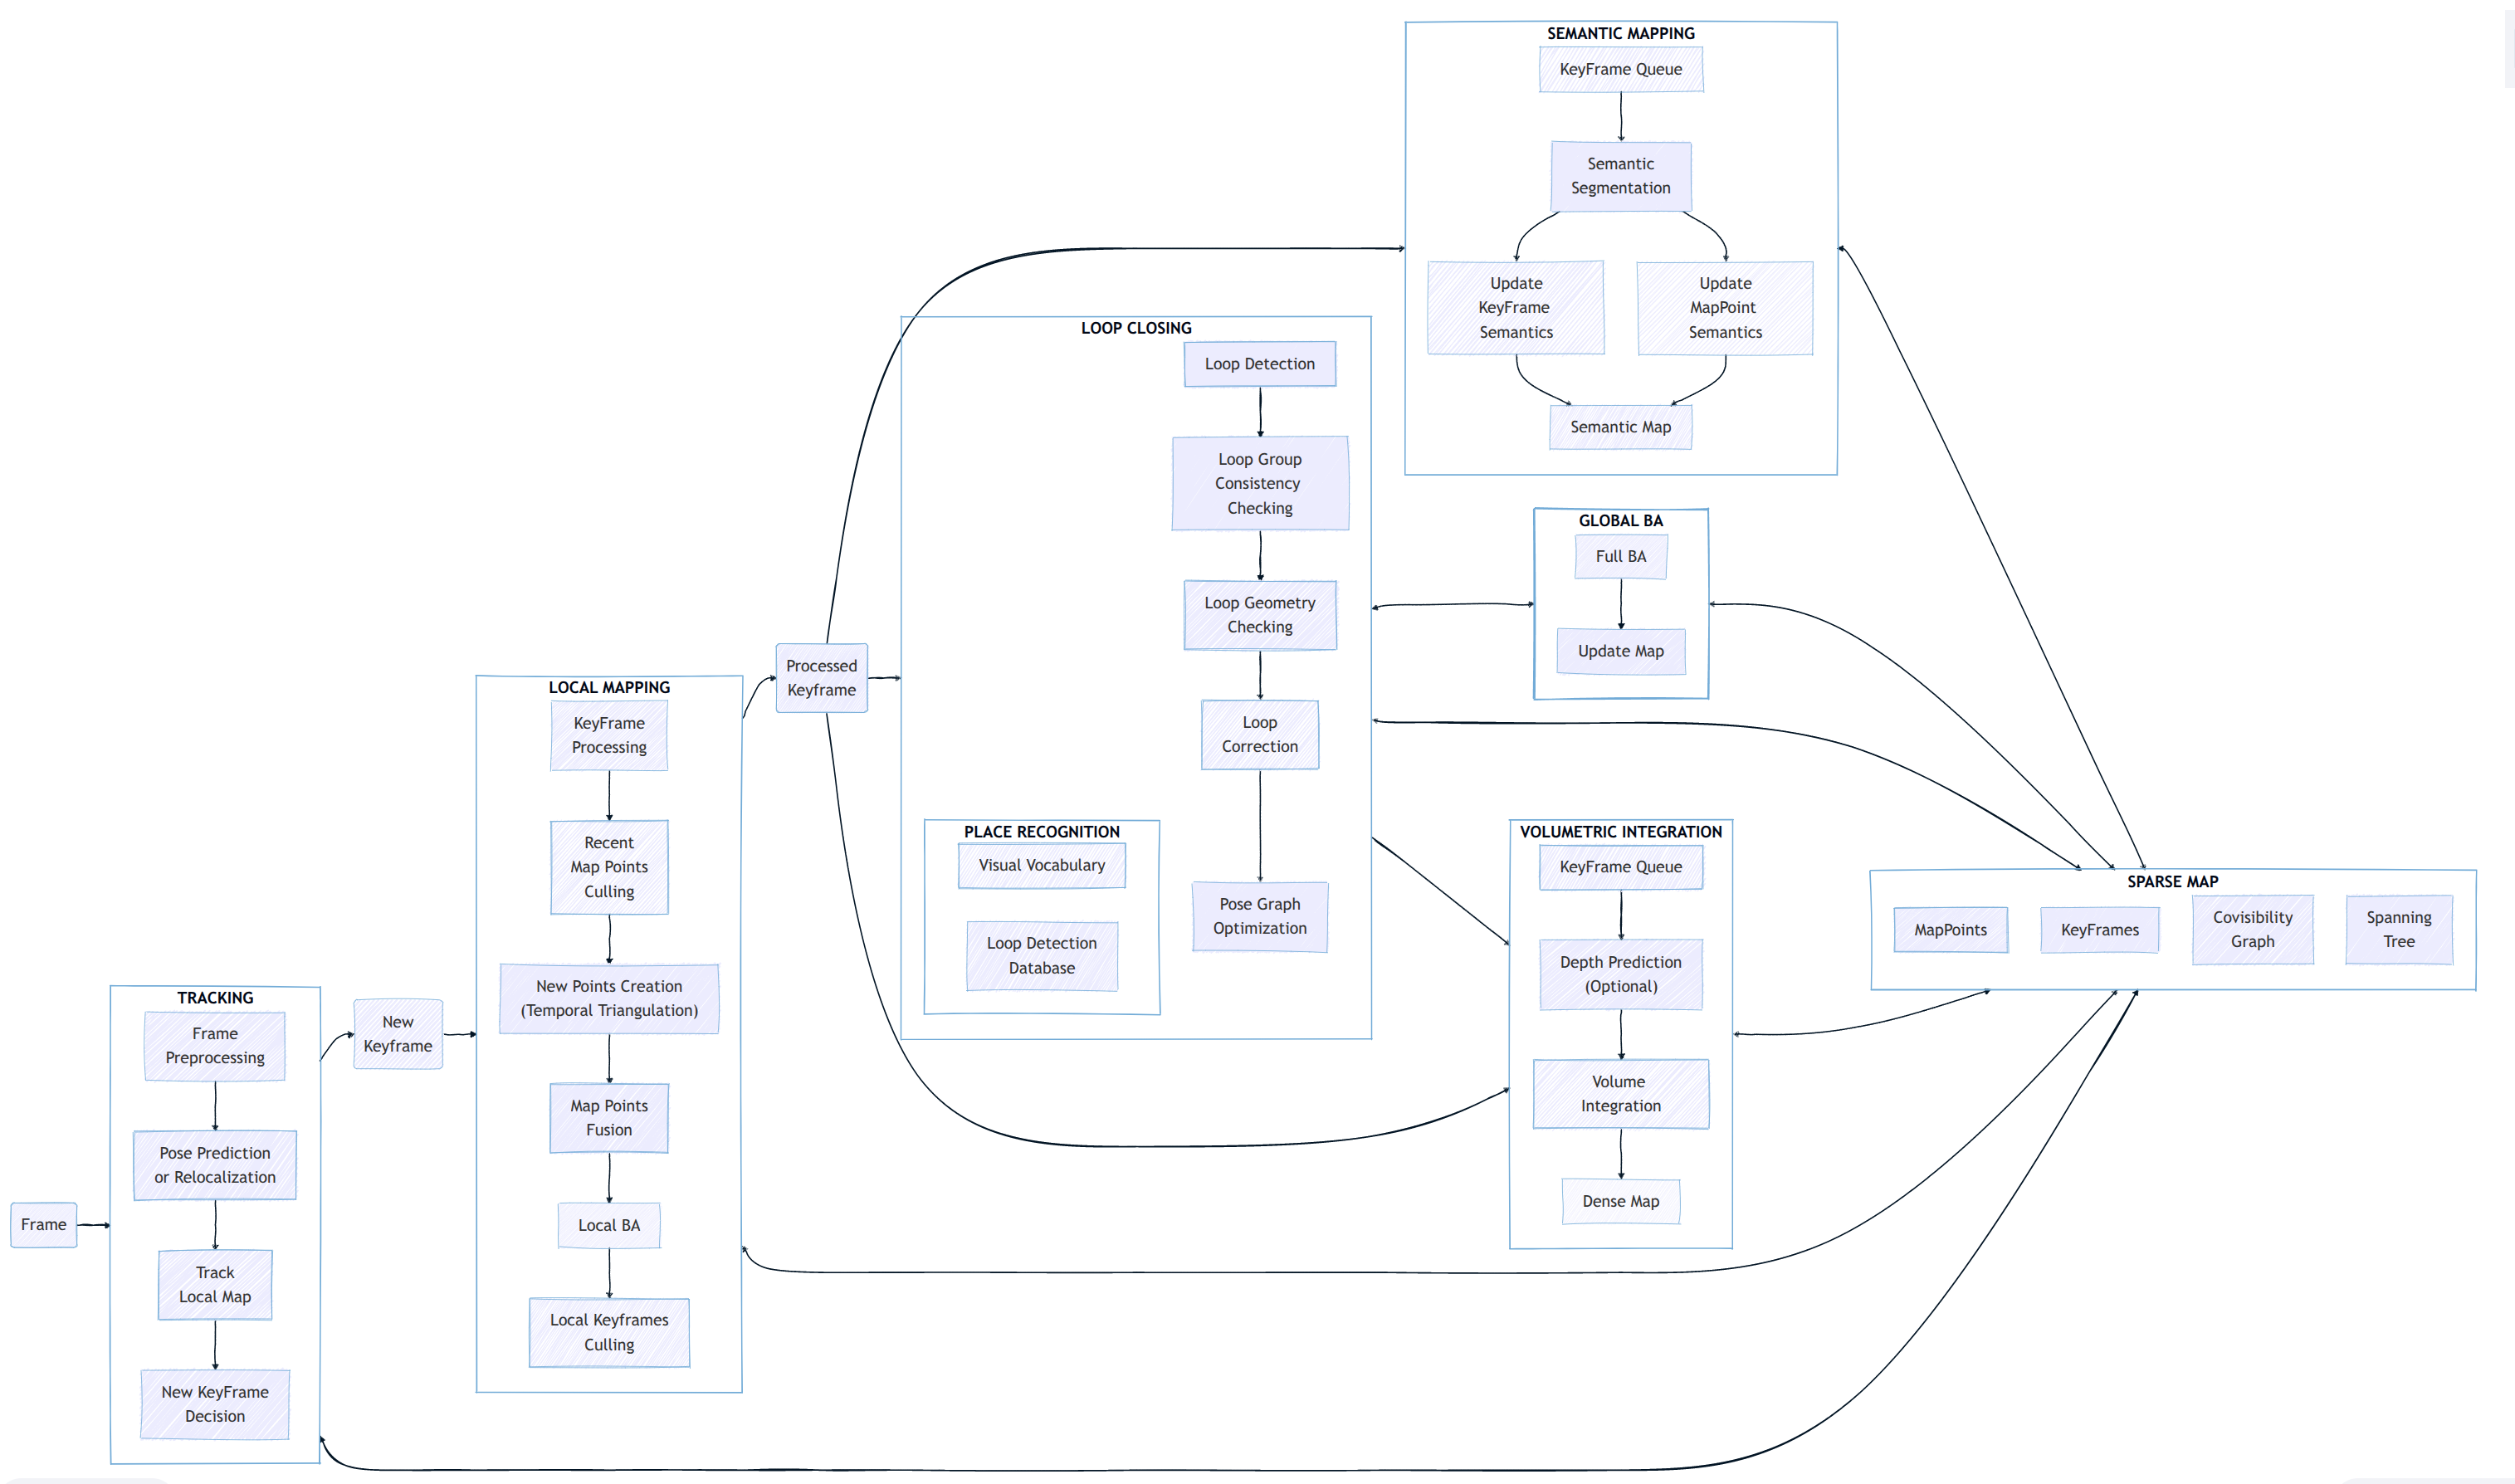
\includegraphics[width=\textwidth]{./images/slam_workflow.png}
\end{center}

\subsection{SLAM Components}
\begin{center}
    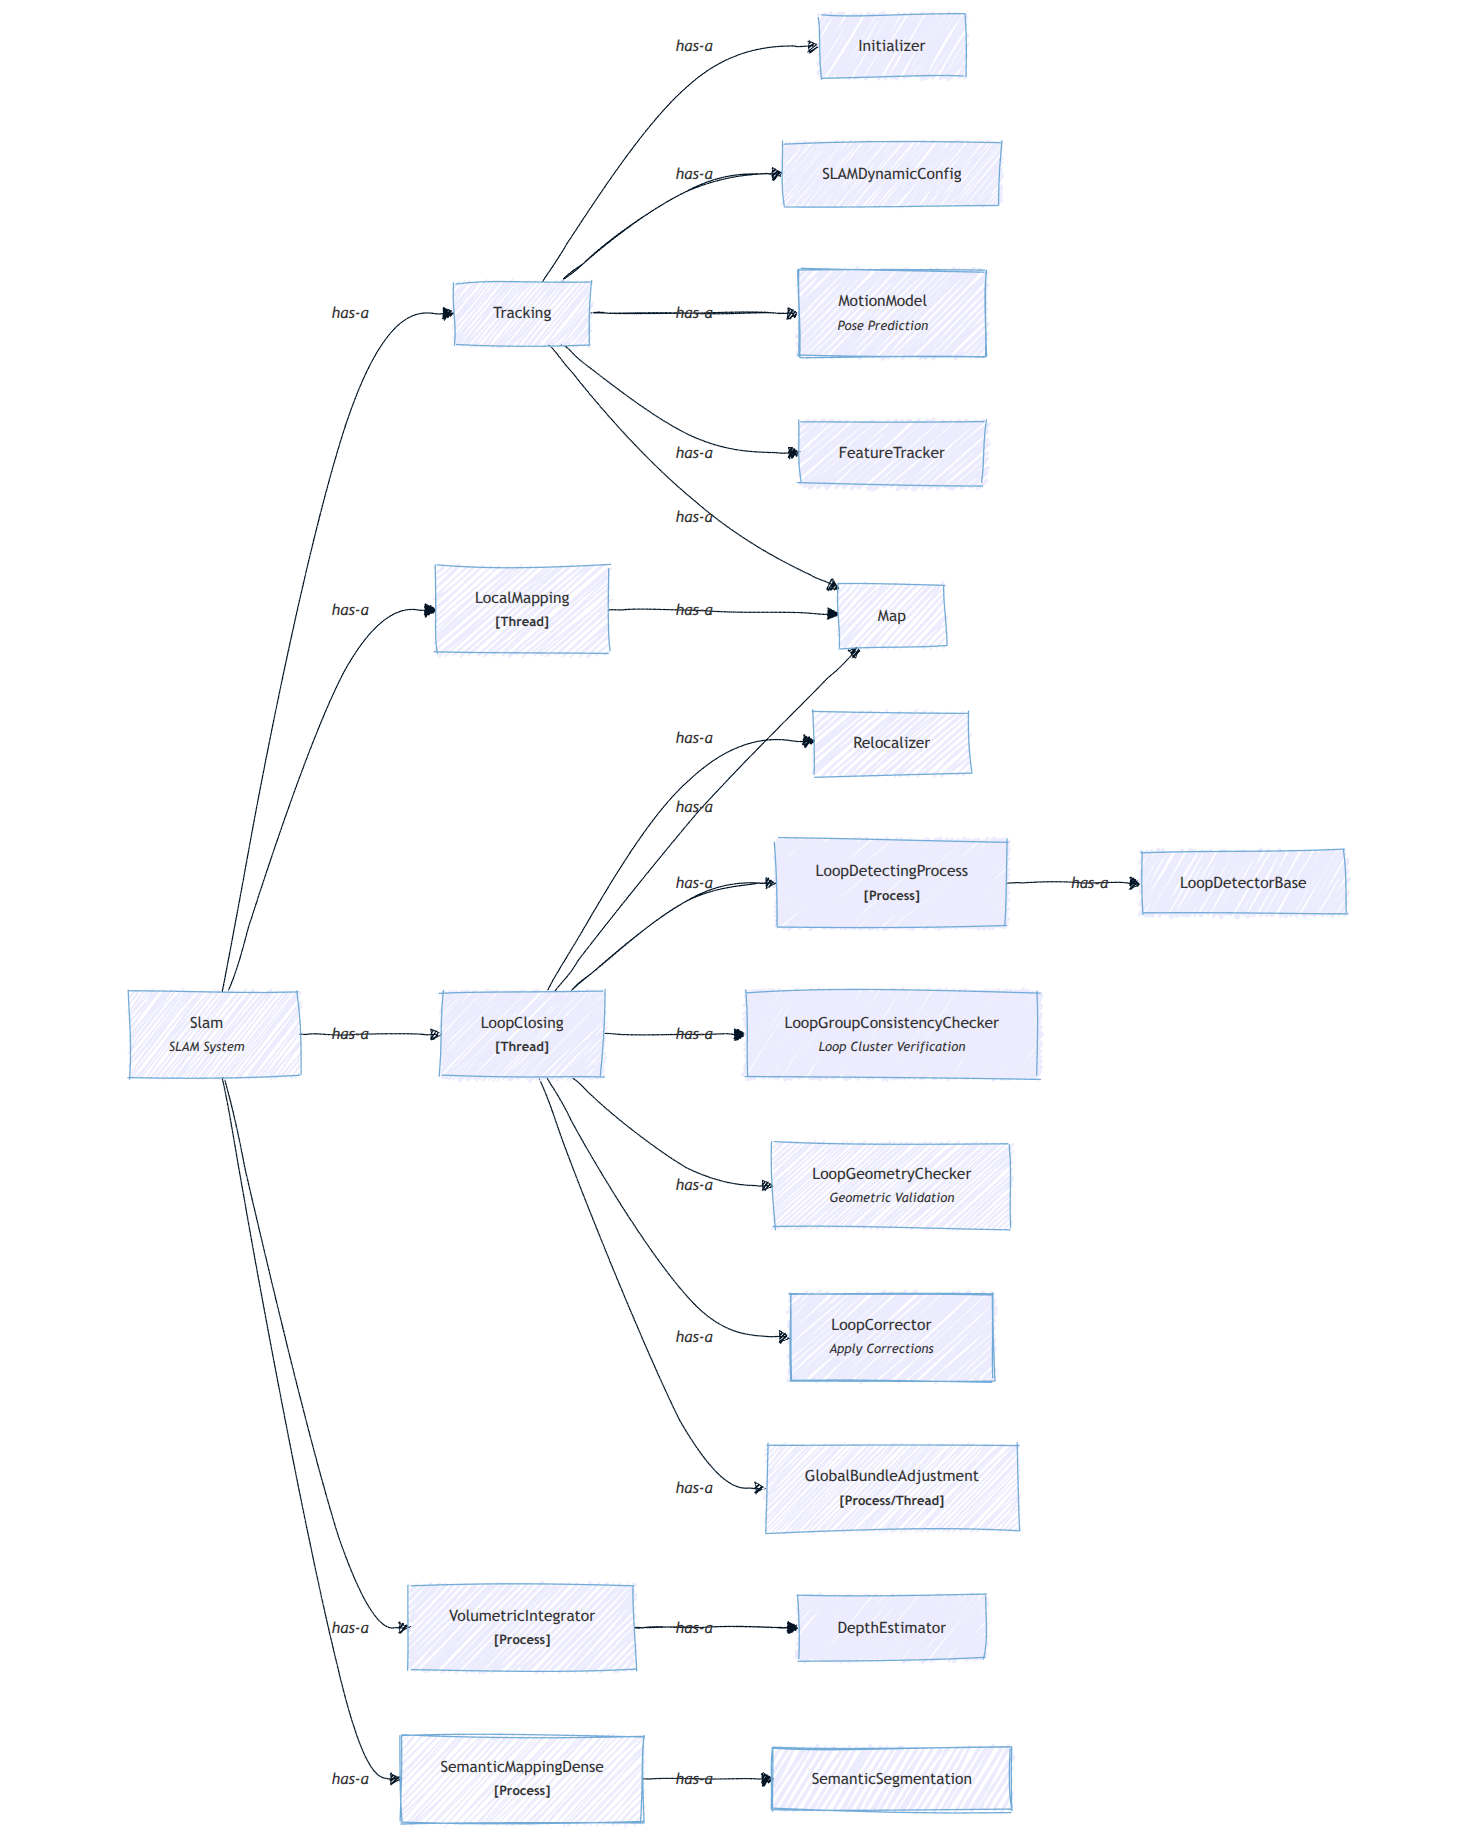
\includegraphics[width=0.8\textwidth]{./images/slam_components.png}
\end{center}

\textbf{Note}: You might be wondering why I used \textbf{Processes} instead of \textbf{Threads} in some cases. The reason is that, at least in Python 3.8 (the version supporting pySLAM), only one thread can execute at a time within a single process due to the Global Interpreter Lock (GIL). On the other hand, using multiprocessing (separate processes that do not share the GIL) enables better parallelism. See this nice \href{https://www.theserverside.com/blog/Coffee-Talk-Java-News-Stories-and-Opinions/Is-Pythons-GIL-the-software-worlds-biggest-blunder}{post}.

\subsection{Main System Components}

\textbf{Feature Tracker}
\begin{center}
    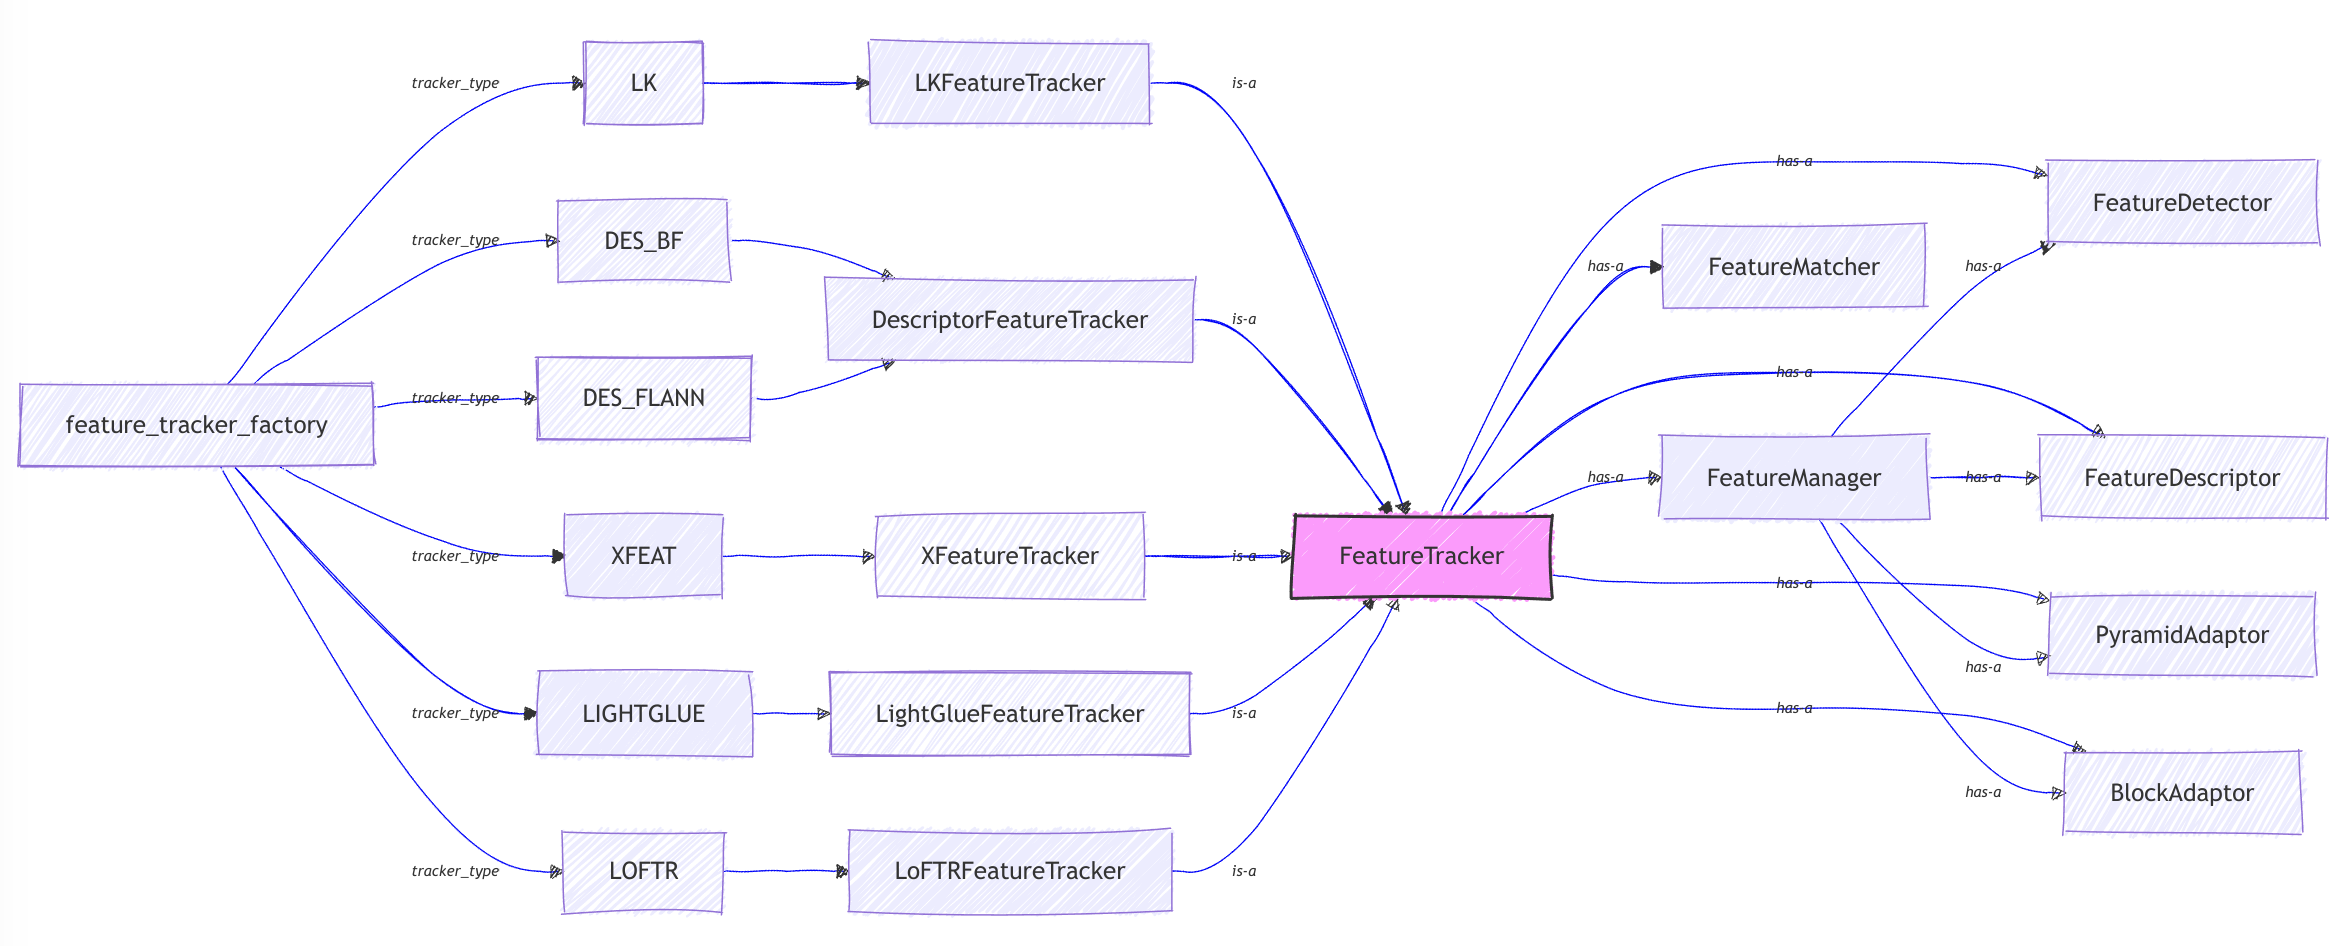
\includegraphics[width=0.8\textwidth]{./images/feature_tracker.png}
\end{center}

\textbf{Feature Matcher}
\begin{center}
    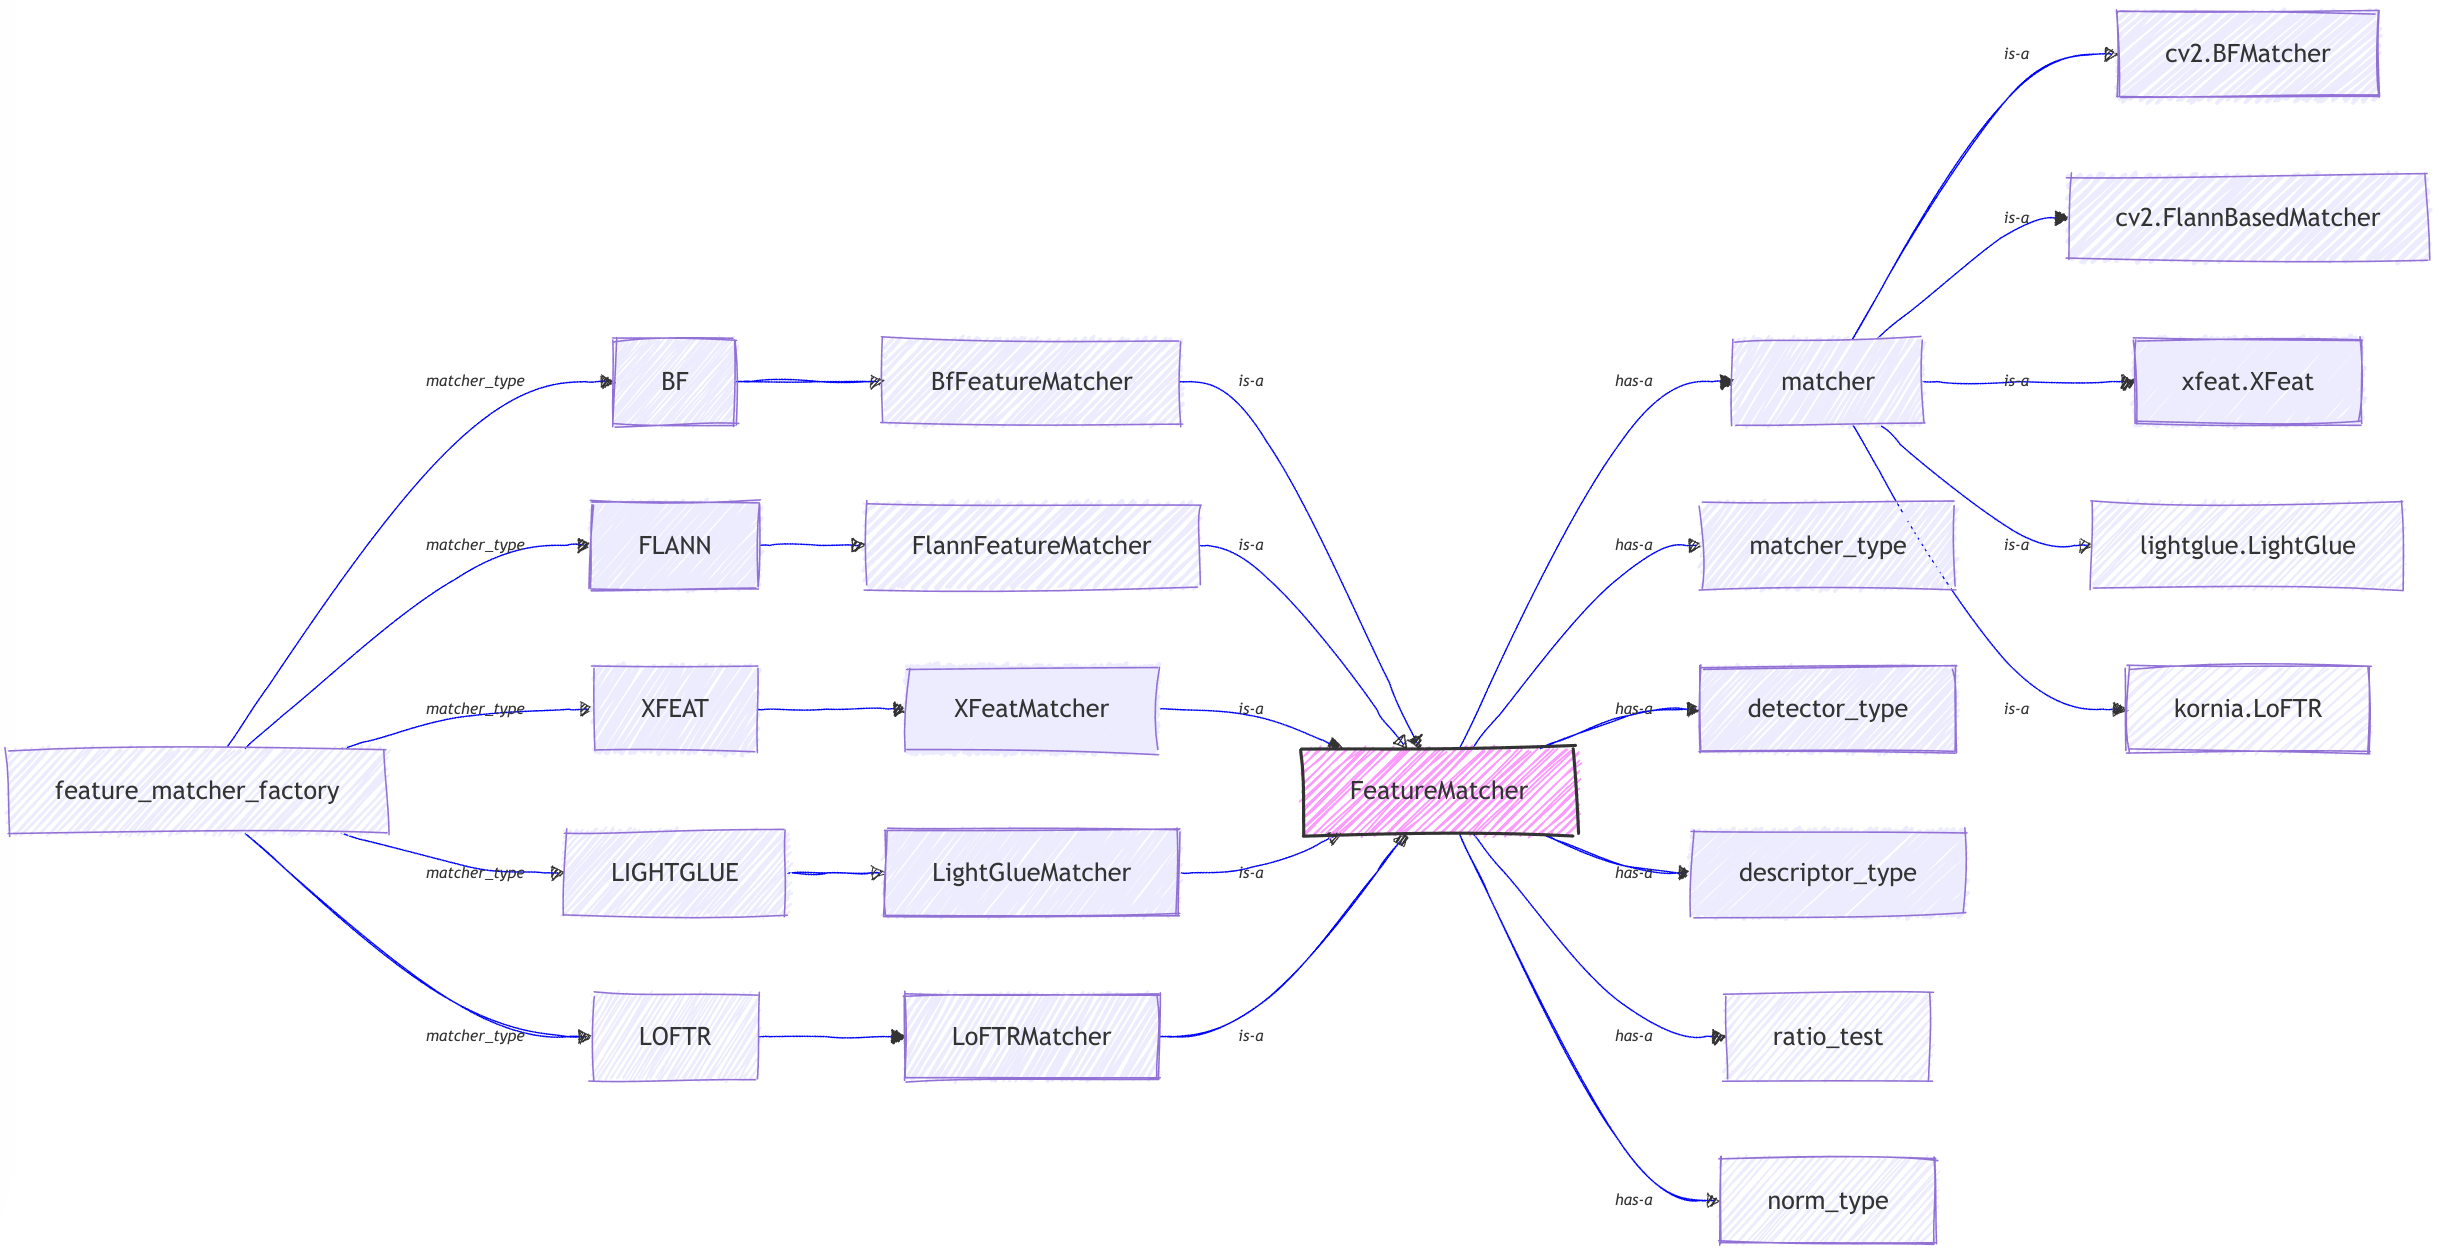
\includegraphics[width=0.8\textwidth]{./images/feature_matcher.png}
\end{center}

\textbf{Loop Detector}
\begin{center}
    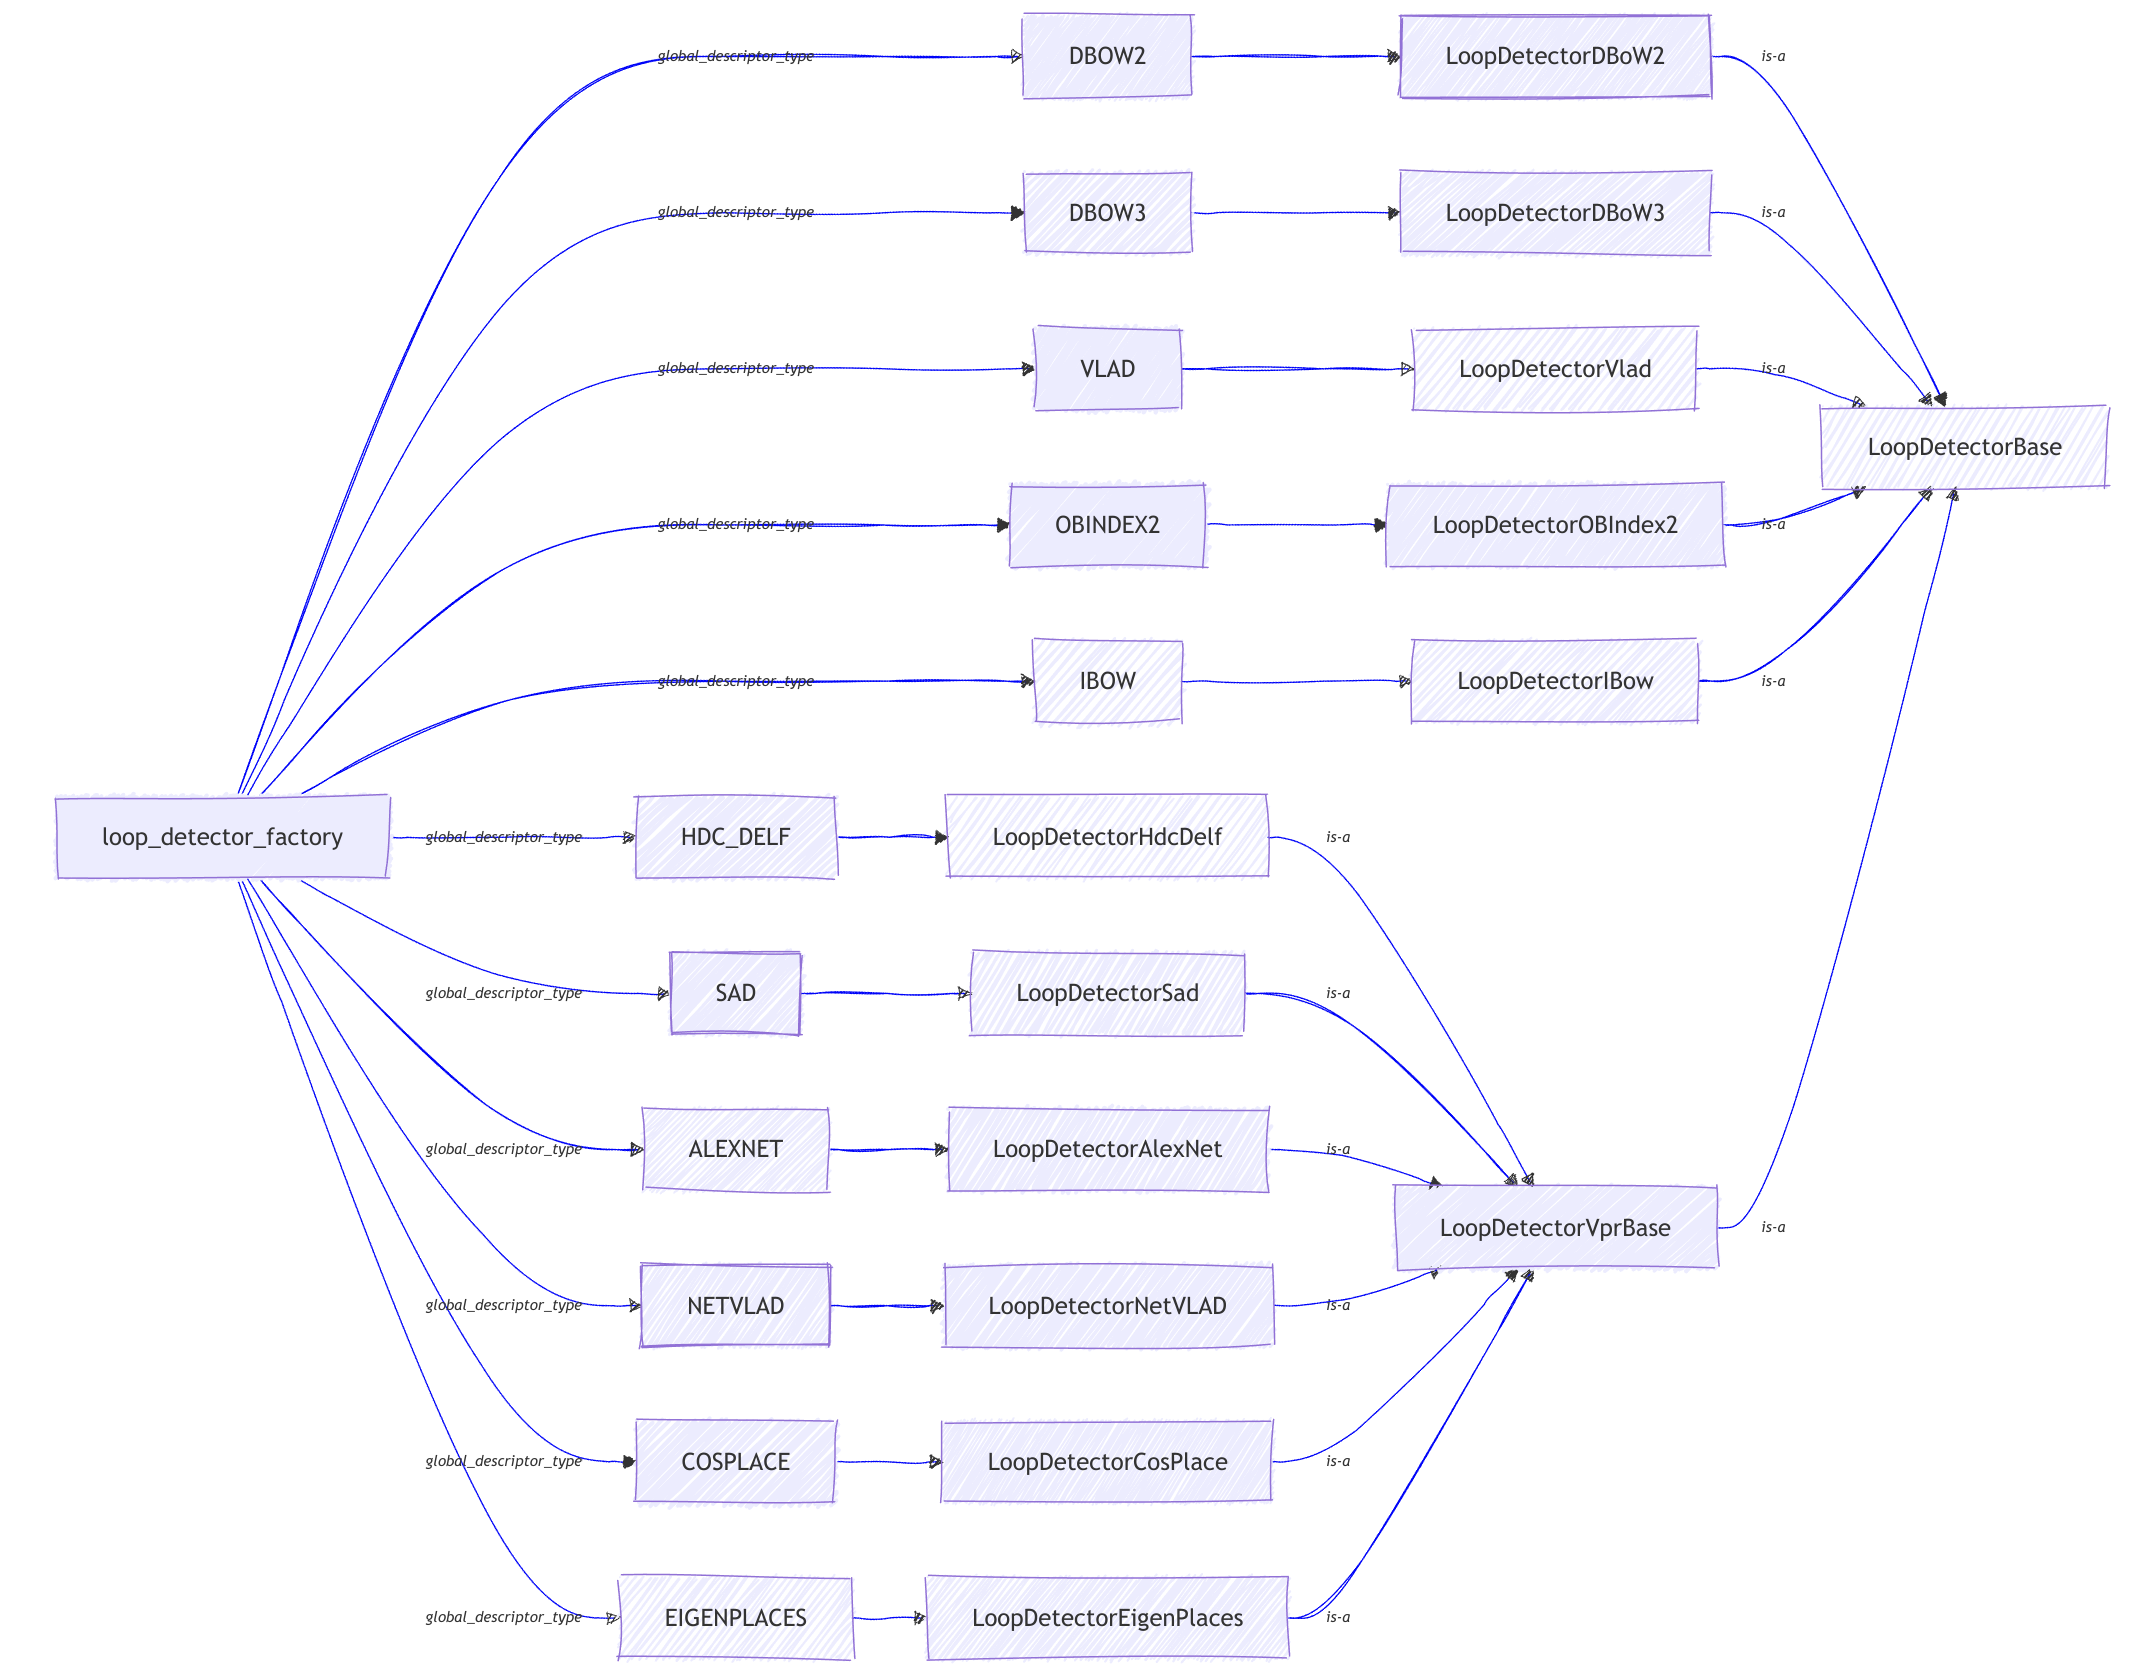
\includegraphics[width=0.8\textwidth]{./images/loop_detector.png}
\end{center}

\textbf{Depth Estimator}
\begin{center}
    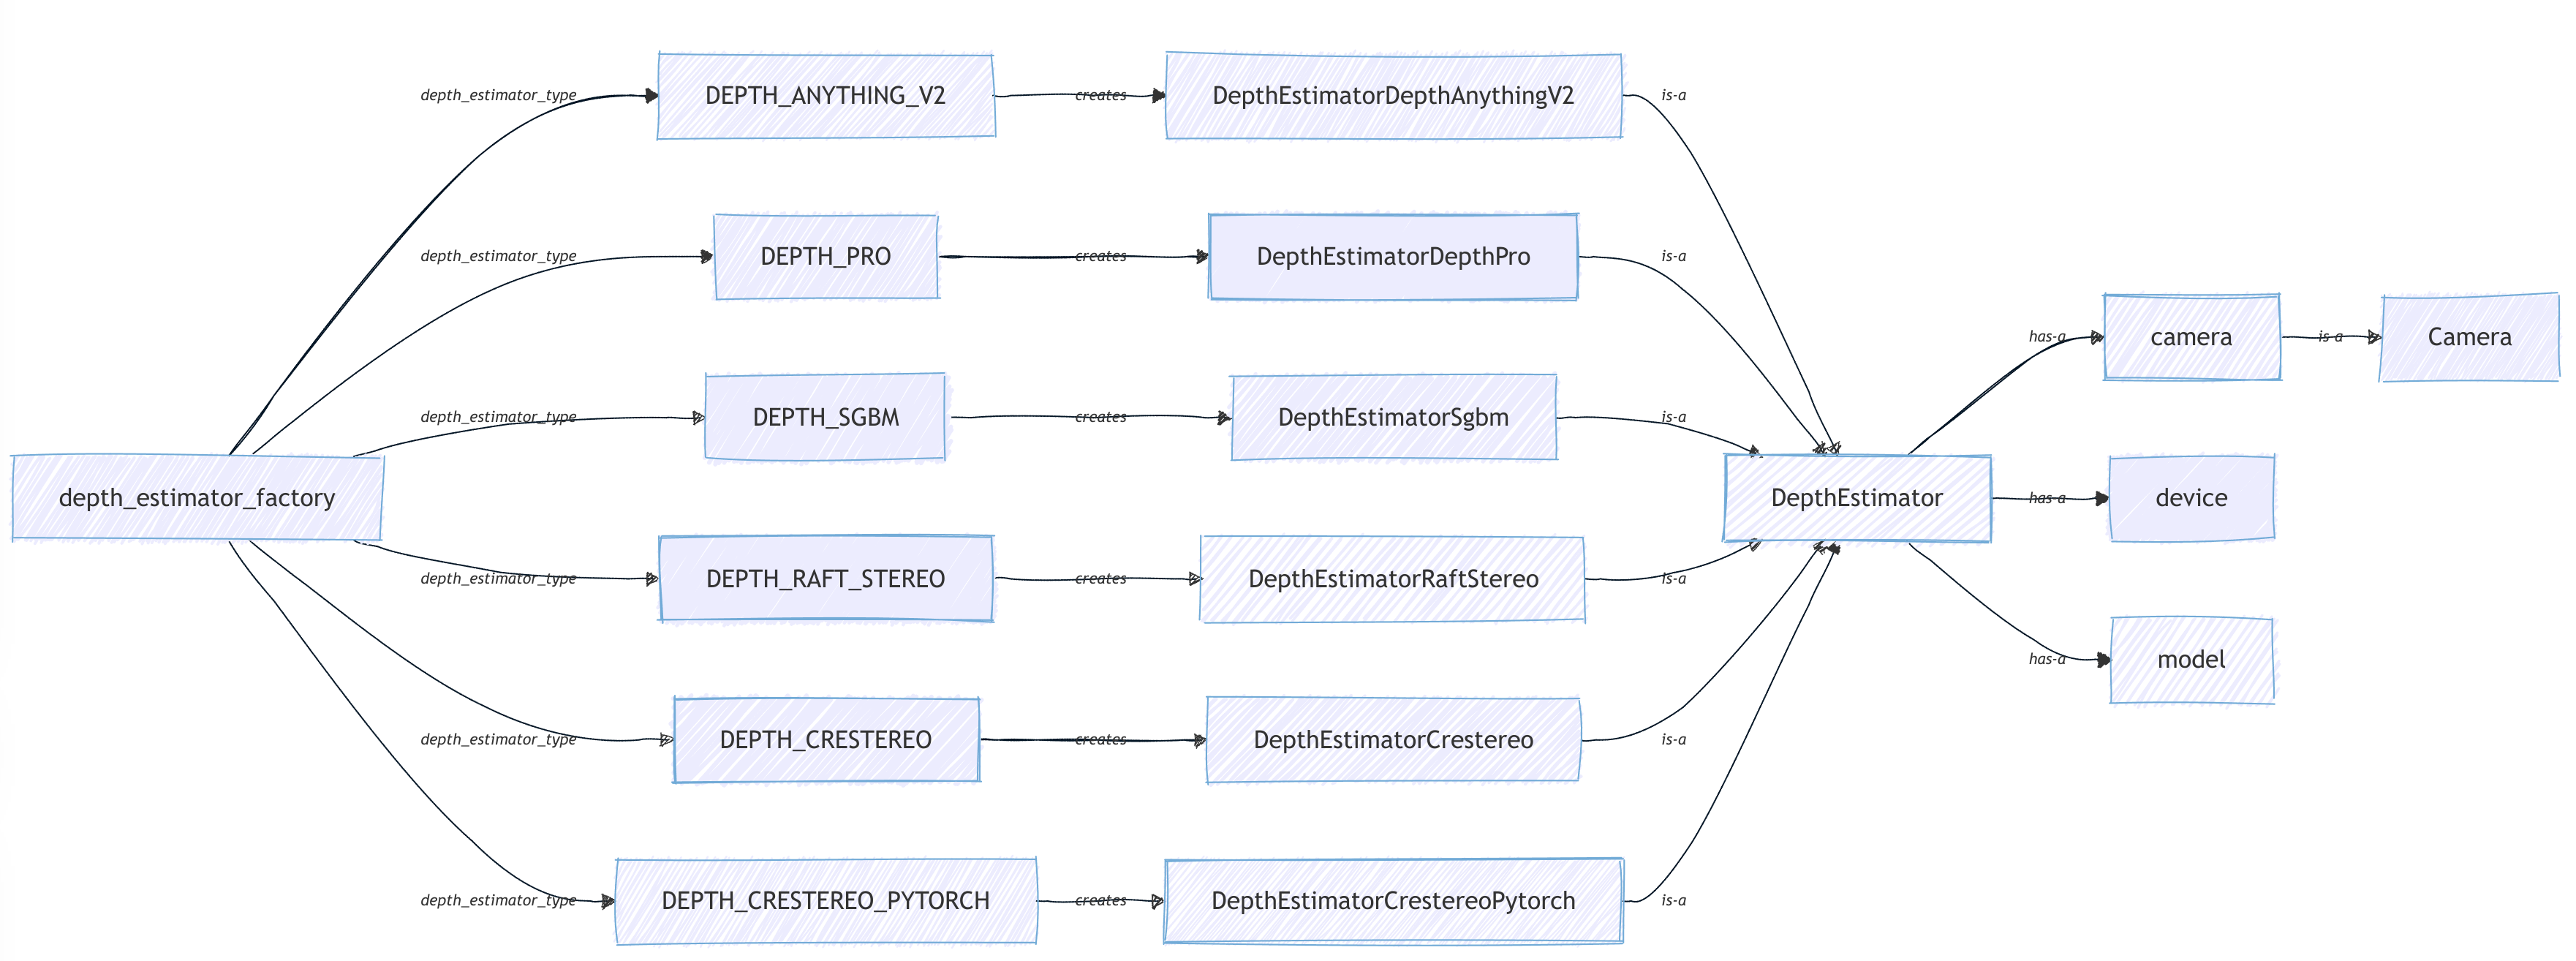
\includegraphics[width=0.8\textwidth]{./images/depth_estimator.png}
\end{center}

\subsection{Volumetric Integrator}
\begin{center}
    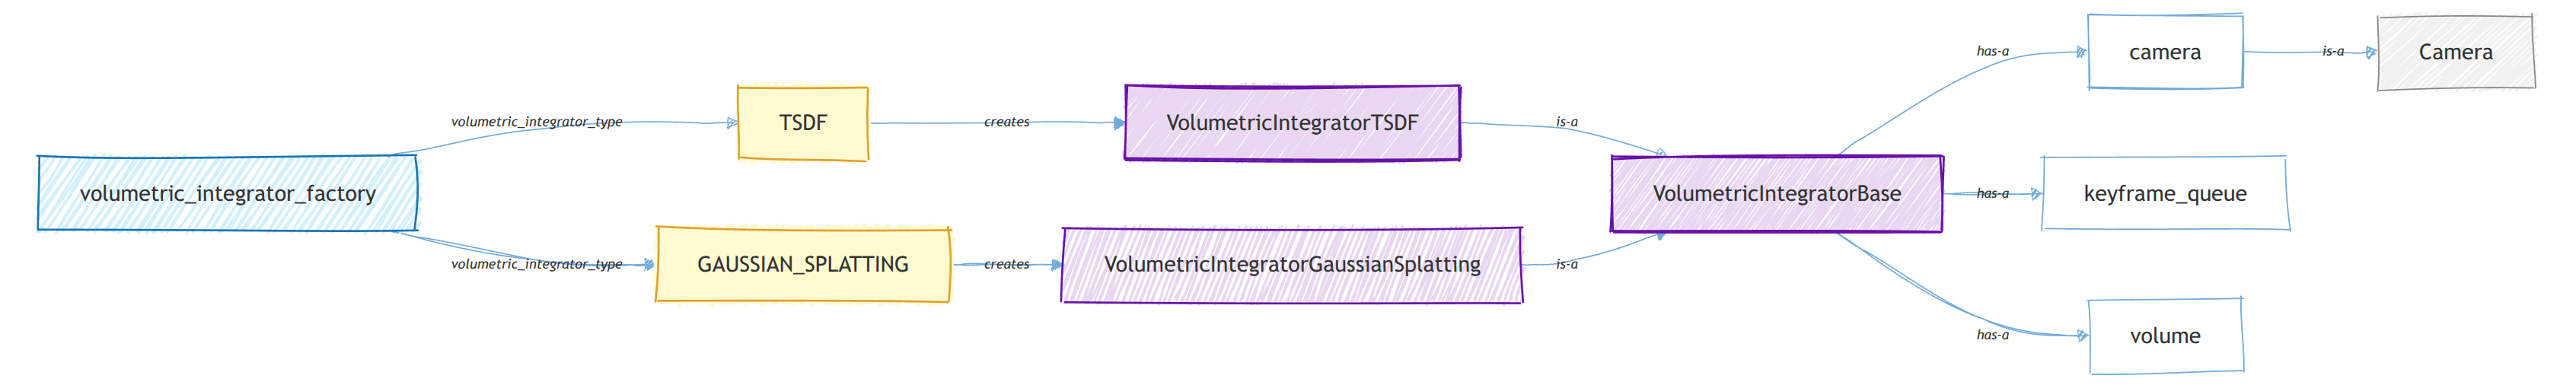
\includegraphics[width=0.8\textwidth]{./images/volumetric_integrator.png}
\end{center}

\hypertarget{usage}{%
\section{Usage}\label{usage}}

Once you have run the script \texttt{install\_all\_venv.sh} (follow the
instructions above according to your OS), you can open a new terminal
and start testing the basic \textbf{Visual Odometry} (VO):\\

\begin{scriptsize}
\begin{Shaded}
\begin{Highlighting}[]
\NormalTok{$ }\BuiltInTok{.} \ExtensionTok{pyenv-activate.sh}   \CommentTok{#  Activate pyslam python virtual environment. This is only needed once in a new terminal.}
\NormalTok{$ }\ExtensionTok{./main_vo.py}
\end{Highlighting}
\end{Shaded}
\end{scriptsize}


This will process a default
\href{http://www.cvlibs.net/datasets/kitti/eval_odometry.php}{KITTI}
video (available in the folder \texttt{data/videos}) by using its
corresponding camera calibration file (available in the folder
\texttt{settings}), and its groundtruth (available in the same
\texttt{data/videos} folder). If matplotlib windows are used, you can
stop \texttt{main\_vo.py} by focusing/clicking on one of them and
pressing the key `Q'. As explained above, this very \emph{basic} script
\texttt{main\_vo.py} \textbf{strictly requires a ground truth}.

Similarly, you can test the \textbf{full SLAM} by running
\texttt{main\_slam.py}:\\

\begin{scriptsize}
\begin{Shaded}
\begin{Highlighting}[]
\NormalTok{$ }\BuiltInTok{.} \ExtensionTok{pyenv-activate.sh}   \CommentTok{#  Activate pyslam python virtual environment. This is only needed once in a new terminal.}
\NormalTok{$ }\ExtensionTok{./main_slam.py}
\end{Highlighting}
\end{Shaded}
\end{scriptsize}

This will process the same default
\href{(http://www.cvlibs.net/datasets/kitti/eval_odometry.php)}{KITTI}
video (available in the folder \texttt{data/videos}) by using its
corresponding camera calibration file (available in the folder
\texttt{settings}). You can stop it by focusing/clicking on one of the
opened windows and pressing the key `Q' or closing the 3D pangolin GUI.

With both scripts, in order to process a different \textbf{dataset}, you
need to update the file \texttt{config.yaml}: * Select your dataset
\texttt{type} in the section \texttt{DATASET} (further details in the
section \emph{\protect\hyperlink{datasets}{Datasets}} below for further
details). This identifies a corresponding dataset section
(e.g.~\texttt{KITTI\_DATASET}, \texttt{TUM\_DATASET}, etc). * Select the
\texttt{sensor\_type} (\texttt{mono}, \texttt{stereo}, \texttt{rgbd}) in
the chosen dataset section.\\
* Select the camera \texttt{settings} file in the dataset section
(further details in the section
\emph{\protect\hyperlink{camera-settings}{Camera Settings}} below). *
The \texttt{groudtruth\_file} accordingly (further details in the
section \emph{\protect\hyperlink{datasets}{Datasets}} below and check
the files \texttt{io/ground\_truth.py} and
\texttt{io/convert\_groundtruth.py}).

\hypertarget{feature-tracking}{%
\subsection{Feature tracking}\label{feature-tracking}}

If you just want to test the basic feature tracking capabilities
(\emph{feature detector} + \emph{feature descriptor} + \emph{feature
matcher}) and get a taste of the different available local features, run \\

\begin{scriptsize}
\begin{Shaded}
\begin{Highlighting}[]
\NormalTok{$ }\BuiltInTok{.} \ExtensionTok{pyenv-activate.sh}   \CommentTok{#  Activate pyslam python virtual environment. This is only needed once in a new terminal.}
\NormalTok{$}\ExtensionTok{./main_feature_matching.py}
\end{Highlighting}
\end{Shaded}
\end{scriptsize}


In any of the above scripts, you can choose any detector/descriptor
among \emph{ORB}, \emph{SIFT}, \emph{SURF}, \emph{BRISK}, \emph{AKAZE},
\emph{SuperPoint}, etc. (see the section
\emph{\protect\hyperlink{supported-local-features}{Supported Local
Features}} below for further information).

Some basic examples are available in the subfolder
\texttt{test/loopclosing}. In particular, as for feature
detection/description, you may want to take a look at
\href{./test/cv/test_feature_manager.py}{test/cv/test\_feature\_manager.py}
too.

\hypertarget{loop-closing}{%
\subsection{Loop closing}\label{loop-closing}}

Different \protect\hyperlink{loop-closing}{loop closing methods} are
available, combining
\protect\hyperlink{local-descriptor-aggregation-methods}{aggregation
methods} and \protect\hyperlink{global-descriptors}{global descriptors}.

While running full SLAM, loop closing is enabled by default and can be
disabled by setting \texttt{kUseLoopClosing=False} in
\texttt{config\_parameters.py}. Configuration options can be found in
\url{loop_closing/loop_detector_configs.py}.

\textbf{Examples}: Start with the examples in \texttt{test/loopclosing},
such as
\href{./test/loopclosing/test_loop_detector.py}{test/loopclosing/test\_loop\_detector.py}.

\hypertarget{vocabulary-management}{%
\paragraph{Vocabulary management}\label{vocabulary-management}}

\texttt{DBoW2}, \texttt{DBoW3}, and \texttt{VLAD} require pre-trained
vocabularies. ORB-based vocabularies are automatically downloaded in the
\texttt{data} folder (see \url{loop_closing/loop_detector_configs.py}).

To create a new vocabulary, follow these steps:

\begin{enumerate}
\def\labelenumi{\arabic{enumi}.}
\item
  \textbf{Generate an array of descriptors}: Use the script \\
  \texttt{test/loopclosing/test\_gen\_des\_array\_from\_imgs.py} to
  generate the array of descriptors that will be used to train the new
  vocabulary. Select your desired descriptor type via the tracker
  configuration.
\item
  \textbf{DBOW vocabulary generation}: Train your target DBOW vocabulary
  by using the script
  \texttt{test/loopclosing/test\_gen\_dbow\_voc\_from\_des\_array.py}.
\item
  \textbf{VLAD vocabulary generation}: Train your target VLAD
  ``vocabulary'' by using the script
  \texttt{test/loopclosing/test\_gen\_vlad\_voc\_from\_des\_array.py}.
\end{enumerate}

\hypertarget{vocabulary-free-loop-closing}{%
\paragraph{Vocabulary-free loop
closing}\label{vocabulary-free-loop-closing}}

Most methods do not require pre-trained vocabularies. Specifically: -
\texttt{iBoW} and \texttt{OBindex2}: These methods incrementally build
bags of binary words and, if needed, convert (front-end) non-binary
descriptors into binary ones. - Others: Methods like \texttt{HDC\_DELF},
\texttt{SAD}, \texttt{AlexNet}, \texttt{NetVLAD}, \texttt{CosPlace}, and
\texttt{EigenPlaces} directly extract global descriptors and process
them using dedicated aggregators, independently from the used front-end
descriptors.

As mentioned above, only \texttt{DBoW2}, \texttt{DBoW3}, and
\texttt{VLAD} require pre-trained vocabularies.

\hypertarget{volumetric-reconstruction}{%
\subsection{Volumetric
reconstruction}\label{volumetric-reconstruction}}

\hypertarget{dense-reconstruction-while-running-slam}{%
\paragraph{Dense reconstruction while running
SLAM}\label{dense-reconstruction-while-running-slam}}

The SLAM back-end hosts a volumetric reconstruction pipeline. This is
disabled by default. You can enable it by setting
\texttt{kUseVolumetricIntegration=True} and selecting your preferred
method \texttt{kVolumetricIntegrationType} in
\texttt{config\_parameters.py}. At present, two methods are available:
\texttt{TSDF} and \texttt{GAUSSIAN\_SPLATTING} (see
\url{dense/volumetric_integrator_factory.py}). Note that you need CUDA
in order to run \texttt{GAUSSIAN\_SPLATTING} method.

At present, the volumetric reconstruction pipeline works with: - RGBD
datasets - When a \protect\hyperlink{depth-prediction}{depth estimator}
is used in the back-end or front-end and a depth prediction/estimation
gets available for each processed keyframe.

If you want a mesh as output then set
\texttt{kVolumetricIntegrationExtractMesh=True} in
\texttt{config\_parameters.py}.

\hypertarget{reload-a-saved-sparse-map-and-perform-dense-reconstruction}{%
\paragraph{Reload a saved sparse map and perform dense
reconstruction}\label{reload-a-saved-sparse-map-and-perform-dense-reconstruction}}

Use the script \texttt{main\_map\_dense\_reconstruction.py} to reload a
saved sparse map and to perform dense reconstruction by using its posed
keyframes as input. You can select your preferred dense reconstruction
method directly in the script.

\begin{itemize}
\tightlist
\item
  To check what the volumetric integrator is doing, run in another shell
  \texttt{tail\ -f\ logs/volumetric\_integrator.log} (from repository
  root folder).
\item
  To save the obtained dense and sparse maps, press the \texttt{Save}
  button on the GUI.
\end{itemize}

\hypertarget{reload-and-check-your-dense-reconstruction}{%
\paragraph{Reload and check your dense
reconstruction}\label{reload-and-check-your-dense-reconstruction}}

You can check the output pointcloud/mesh by using
\href{https://www.cloudcompare.org/}{CloudCompare}.

In the case of a saved Gaussian splatting model, you can visualize it
by: 
\begin{enumerate}
\item Using the
\href{https://playcanvas.com/supersplat/editor}{superslat editor} (drag
and drop the saved Gaussian splatting \texttt{.ply} pointcloud in the
editor interface). 

\item Getting into the folder
\texttt{test/gaussian\_splatting} and running:\\
\texttt{\$\ python\ test\_gsm.py\ -\/-load\ \textless{}gs\_checkpoint\_path\textgreater{}}~\\
%The \texttt{\textless{}gs\_checkpoint\_path\textgreater{}} is expected
%to have the following structure:\\
%\texttt{bash\ \ \ \ \ ├──\ gs\_checkpoint\_path\ \ \ \ \ \ \ \ \ ├──\ pointcloud\ \ \ \#\ folder\ containing\ different\ subfolders,\ each\ one\ with\ a\ saved\ .ply\ econding\ the\ gaussian\ splatting\ model\ at\ a\ specific\ iteration/checkpoint\ \ \ \ \ \ \ \ \ ├──\ last\_camera.json\ \ \ \ \ \ \ \ \ ├──\ config.yml}
\end{enumerate}

\hypertarget{controlling-the-spatial-distribution-of-keyframe-fov-centers}{%
\paragraph{Controlling the spatial distribution of keyframe FOV
centers}\label{controlling-the-spatial-distribution-of-keyframe-fov-centers}}

If you are targeting volumetric reconstruction while running SLAM, you
can enable a \textbf{keyframe generation policy} designed to manage the
spatial distribution of keyframe field-of-view (FOV) centers. The
\emph{FOV center of a camera} is defined as the backprojection of its
image center, calculated using the median depth of the frame. With this
policy, a new keyframe is generated only if its FOV center is farther
than a predefined distance from the nearest existing keyframe's FOV
center. You can enable this policy by setting the following parameters
in the yaml setting:\\

\begin{scriptsize}
\begin{Shaded}
\begin{Highlighting}[]
\FunctionTok{KeyFrame.useFovCentersBasedGeneration:}\AttributeTok{ }\DecValTok{1}\AttributeTok{  }\CommentTok{# compute 3D fov centers of camera frames by using median depth and use their distances to control keyframe generation}
\FunctionTok{KeyFrame.maxFovCentersDistance:}\AttributeTok{ }\FloatTok{0.2}\AttributeTok{       }\CommentTok{# max distance between fov centers in order to generate a keyframe}
\end{Highlighting}
\end{Shaded}
\end{scriptsize}


\hypertarget{depth-prediction}{%
\subsection{Depth prediction}\label{depth-prediction}}

The available depth prediction models can be utilized both in the SLAM
back-end and front-end. - Back-end: Depth prediction can be enabled in
the \protect\hyperlink{volumetric-reconstruction-pipeline}{volumetric
reconstruction} pipeline by setting the parameter
\texttt{kVolumetricIntegrationUseDepthEstimator=True} and selecting your
preferred \texttt{kVolumetricIntegrationDepthEstimatorType} in
\texttt{config\_parameters.py}. - Front-end: Depth prediction can be
enabled in the front-end by setting the parameter
\texttt{kUseDepthEstimatorInFrontEnd} in \texttt{config\_parameters.py}.
This feature estimates depth images from input color images to emulate a
RGBD camera. Please, note this functionality is still
\emph{experimental} at present time.

Refer to the file
\texttt{depth\_estimation/depth\_estimator\_factory.py} for further
details. Both stereo and monocular prediction approaches are supported.
You can test depth prediction/estimation by using the script
\texttt{main\_depth\_prediction.py}.

\textbf{Notes}: * In the case of a monocular SLAM configuration, do NOT
use depth prediction in the back-end volumetric integration: The SLAM
(fake) scale will conflict with the absolute metric scale of depth
predictions. With monocular datasets, enable depth prediction to run in
the front-end. - The depth inference may be very slow (for instance,
with DepthPro it takes \textasciitilde{}1s per image on my machine).
Therefore, the resulting volumetric reconstruction pipeline may be very
slow.

\hypertarget{save-the-a-map}{%
\subsection{Save the a map}\label{save-the-a-map}}

When you run the script \texttt{main\_slam.py}
(\texttt{main\_map\_dense\_reconstruction.py}): - You can save the
current map state by pressing the button \texttt{Save} on the GUI. This
saves the current map along with front-end, and backend configurations
into the default folder \texttt{results/slam\_state}
(\texttt{results/slam\_state\_dense\_reconstruction}). - To change the
default saving path, open \texttt{config.yaml} and update target
\texttt{folder\_path} in the section:
\texttt{bash\ \ \ SYSTEM\_STATE:\ \ \ \ \ folder\_path:\ results/slam\_state\ \ \ \#\ default\ folder\ path\ (relative\ to\ repository\ root)\ where\ the\ system\ state\ is\ saved\ or\ reloaded}

\hypertarget{reload-a-saved-map-and-relocalize-in-it}{%
\subsection{Reload a saved map and relocalize in
it}\label{reload-a-saved-map-and-relocalize-in-it}}

\begin{itemize}
\item
  A saved map can be loaded and visualized in the GUI by running: \\

\begin{scriptsize}
\begin{Shaded}
\begin{Highlighting}[]
\NormalTok{$ }\BuiltInTok{.} \ExtensionTok{pyenv-activate.sh}   \CommentTok{#  Activate pyslam python virtual environment. This is only needed once in a new terminal.}
\NormalTok{$ }\ExtensionTok{./main_map_viewer.py}  \CommentTok{#  Use the --path options to change the input path}
\end{Highlighting}
\end{Shaded}

\end{scriptsize}

\item
  To enable map reloading and relocalization when running
  \texttt{main\_slam.py}, open \texttt{config.yaml} and set \\

\begin{scriptsize}
\begin{Shaded}
\begin{Highlighting}[]
\ExtensionTok{SYSTEM_STATE}\NormalTok{:}
  \ExtensionTok{load_state}\NormalTok{: True                  }\CommentTok{# flag to enable SLAM state reloading (map state + loop closing state)}
  \ExtensionTok{folder_path}\NormalTok{: results/slam_state   }\CommentTok{# default folder path (relative to repository root) where the system state is saved or reloaded}
\end{Highlighting}
\end{Shaded}
\end{scriptsize}

\end{itemize}

Note that pressing the \texttt{Save} button saves the current map,
front-end, and backend configurations. Reloading a saved map overwrites
the current system configurations to ensure descriptor compatibility.

\hypertarget{trajectory-saving}{%
\subsection{Trajectory saving}\label{trajectory-saving}}

Estimated trajectories can be saved in three different formats:
\emph{TUM} (The Open Mapping format), \emph{KITTI} (KITTI Odometry
format), and \emph{EuRoC} (EuRoC MAV format). To enable trajectory
saving, open \texttt{config.yaml} and search for the
\texttt{SAVE\_TRAJECTORY}: set \texttt{save\_trajectory:\ True}, select
your \texttt{format\_type} (\texttt{tum}, \texttt{kitti},
\texttt{euroc}), and the output filename. For instance for a
\texttt{tum} format output: \\

\begin{scriptsize}
\begin{Shaded}
\begin{Highlighting}[]
\ExtensionTok{SAVE_TRAJECTORY}\NormalTok{:}
  \ExtensionTok{save_trajectory}\NormalTok{: True}
  \ExtensionTok{format_type}\NormalTok{: tum}
  \ExtensionTok{filename}\NormalTok{: results/kitti_trajectory.txt}
\end{Highlighting}
\end{Shaded}

\end{scriptsize}

\hypertarget{slam-gui}{%
\subsection{SLAM GUI}\label{slam-gui}}

Some quick information about the non-trivial GUI buttons of \texttt{main\_slam.py}:

\begin{itemize}
    \item \texttt{Step}: Enter the \emph{Step by step mode}. Press the button \texttt{Step} a first time to pause. Then, press it again to make the pipeline process a single new frame.

    \item \texttt{Save}: Save the map into the file \texttt{map.json}. You can visualize it back by using the script \texttt{/main\_map\_viewer.py} (as explained above).

    \item \texttt{Reset}: Reset SLAM system.

    \item \texttt{Draw Ground Truth}: If a ground truth dataset is loaded (e.g., from KITTI, TUM, EUROC, or REPLICA), you can visualize it by pressing this button. The ground truth trajectory will be displayed in 3D and progressively aligned (approximately every 30 frames) with the estimated trajectory. The alignment improves as more samples are added to the estimated trajectory. After \textasciitilde{}20 frames, if the button is pressed, a window will appear showing the Cartesian alignment errors (ground truth vs.~estimated trajectory) along the axes.
\end{itemize}

\hypertarget{monitor-the-logs-for-tracking-local-mapping-and-loop-closing-simultaneously}{%
\subsection{Monitor the logs for tracking, local mapping, and loop
closing
simultaneously}\label{monitor-the-logs-for-tracking-local-mapping-and-loop-closing-simultaneously}}

The logs generated by the modules \texttt{local\_mapping.py},
\texttt{loop\_closing.py}, \texttt{loop\_detecting\_process.py}, and
\texttt{global\_bundle\_adjustments.py} are collected in the files
\texttt{local\_mapping.log}, \texttt{loop\_closing.log},
\texttt{loop\_detecting.log}, and \texttt{gba.log}, which are all stored
in the folder \texttt{logs}. For debugging, you can monitor a parallel
flow by running the following command in a separate shell:\\
\texttt{\$\ tail\ -f\ logs/\textless{}log\ file\ name\textgreater{}}~\\
Otherwise, to check all parallel logs with tmux, run:\\
\texttt{\$\ ./scripts/launch\_tmux\_logs.sh}~\\
To launch slam and check all logs in a single tmux, run:\\
\texttt{\$\ ./scripts/launch\_tmux\_slam.sh}~\\
Press \texttt{CTRL+A} and then \texttt{CTRL+Q} to exit from
\texttt{tmux} environment.

\hypertarget{supported-components-and-models}{%
\section{Supported components and
models}\label{supported-components-and-models}}

\hypertarget{supported-local-features}{%
\subsection{Supported local
features}\label{supported-local-features}}

At present time, the following feature \textbf{detectors} are supported:

\begin{itemize}
    \item \href{https://www.edwardrosten.com/work/fast.html}{FAST} \cite{rosten2006machine}
    \item \href{https://ieeexplore.ieee.org/document/323794}{Good features to track} \cite{shi1994good}
    \item \href{http://www.willowgarage.com/sites/default/files/orb_final.pdf}{ORB} \cite{rublee2011orb}
    \item \href{https://github.com/raulmur/ORB_SLAM2}{ORB2} (improvements of ORB-SLAM2 to ORB detector)
    \item \href{https://www.cs.ubc.ca/~lowe/papers/iccv99.pdf}{SIFT} \cite{lowe1999object}
    \item \href{http://people.ee.ethz.ch/~surf/eccv06.pdf}{SURF} \cite{bay2006surf}
    \item \href{https://www.doc.ic.ac.uk/~ajd/Publications/alcantarilla_etal_eccv2012.pdf}{KAZE} \cite{alcantarilla2012kaze}
    \item \href{http://www.bmva.org/bmvc/2013/Papers/paper0013/paper0013.pdf}{AKAZE} \cite{alcantarilla2013fast}
    \item \href{http://www.margaritachli.com/papers/ICCV2011paper.pdf}{BRISK} \cite{leutenegger2011brisk}
    \item \href{http://www.i6.in.tum.de/Main/ResearchAgast}{AGAST}
    \item \href{http://cmp.felk.cvut.cz/~matas/papers/matas-bmvc02.pdf}{MSER} \cite{matas2002robust}
    \item \href{https://link.springer.com/content/pdf/10.1007%2F978-3-540-88693-8_8.pdf}{StarDector/CenSurE}
    \item \href{https://www.robots.ox.ac.uk/~vgg/research/affine/det_eval_files/mikolajczyk_ijcv2004.pdf}{Harris-Laplace}
    \item \href{https://github.com/MagicLeapResearch/SuperPointPretrainedNetwork}{SuperPoint}
    \item \href{https://github.com/mihaidusmanu/d2-net}{D2-Net} \cite{dusmanu2019d2}
    \item \href{https://github.com/tensorflow/models/tree/master/research/delf}{DELF} \cite{noh2017large}
    \item \href{https://github.com/lzx551402/contextdesc}{Contextdesc} \cite{luo2020contextdesc}
    \item \href{https://github.com/vcg-uvic/lf-net-release}{LFNet} \cite{ono2018lf}
    \item \href{https://github.com/naver/r2d2}{R2D2} \cite{revaud2019r2d2}
    \item \href{https://github.com/axelBarroso/Key.Net}{Key.Net} \cite{barroso2020key}
    \item \href{https://arxiv.org/abs/2006.13566}{DISK} \cite{tyszkiewicz2020disk}
    \item \href{https://arxiv.org/abs/2304.03608}{ALIKED} \cite{barroso2023alike}
    \item \href{https://arxiv.org/abs/2404.19174}{Xfeat} \cite{barroso2024xfeat}
    \item \href{https://github.com/axelBarroso/Key.Net}{KeyNetAffNetHardNet} (KeyNet detector + AffNet + HardNet descriptor)
\end{itemize}

The following feature \textbf{descriptors} are supported: 

\begin{itemize}
    \item \href{http://www.willowgarage.com/sites/default/files/orb_final.pdf}{ORB} \cite{rublee2011orb}
    \item \href{https://www.cs.ubc.ca/~lowe/papers/iccv99.pdf}{SIFT} \cite{lowe1999object}
    \item \href{https://www.robots.ox.ac.uk/~vgg/publications/2012/Arandjelovic12/arandjelovic12.pdf}{ROOT SIFT}
    \item \href{http://people.ee.ethz.ch/~surf/eccv06.pdf}{SURF} \cite{bay2006surf}
    \item \href{http://www.bmva.org/bmvc/2013/Papers/paper0013/paper0013.pdf}{AKAZE} \cite{alcantarilla2013fast}
    \item \href{http://www.margaritachli.com/papers/ICCV2011paper.pdf}{BRISK} \cite{leutenegger2011brisk}
    \item \href{https://www.researchgate.net/publication/258848394_FREAK_Fast_retina_keypoint}{FREAK}
    \item \href{https://github.com/MagicLeapResearch/SuperPointPretrainedNetwork}{SuperPoint}
    \item \href{https://github.com/vbalnt/tfeat}{Tfeat}
    \item \href{https://www.labri.fr/perso/vlepetit/pubs/trzcinski_pami15.pdf}{BOOST-DESC} \cite{trzcinski2013boosting}
    \item \href{https://ieeexplore.ieee.org/document/4815264}{DAISY} \cite{tola2010daisy}
    \item \href{https://arxiv.org/abs/1501.03719}{LATCH} \cite{levi2006latch}
    \item \href{https://pdfs.semanticscholar.org/85bd/560cdcbd4f3c24a43678284f485eb2d712d7.pdf}{LUCID}
    \item \href{https://www.robots.ox.ac.uk/~vedaldi/assets/pubs/simonyan14learning.pdf}{VGG} \cite{simonyan2014learning}
    \item \href{https://github.com/DagnyT/hardnet.git}{Hardnet} \cite{mishchuk2017working}
    \item \href{https://github.com/lzx551402/geodesc.git}{GeoDesc} \cite{verdie2018tilde}
    \item \href{https://github.com/yuruntian/SOSNet.git}{SOSNet}
    \item \href{https://github.com/yuruntian/L2-Net}{L2Net}
    \item \href{https://github.com/cvlab-epfl/log-polar-descriptors}{Log-polar descriptor}
    \item \href{https://github.com/mihaidusmanu/d2-net}{D2-Net} \cite{dusmanu2019d2}
    \item \href{https://github.com/tensorflow/models/tree/master/research/delf}{DELF} \cite{noh2017large}
    \item \href{https://github.com/lzx551402/contextdesc}{Contextdesc} \cite{luo2020contextdesc}
    \item \href{https://github.com/vcg-uvic/lf-net-release}{LFNet} \cite{ono2018lf}
    \item \href{https://github.com/naver/r2d2}{R2D2} \cite{revaud2019r2d2}
    \item \href{https://raw.githubusercontent.com/iago-suarez/BEBLID/master/BEBLID_Boosted_Efficient_Binary_Local_Image_Descriptor.pdf}{BEBLID}
    \item \href{https://arxiv.org/abs/2006.13566}{DISK} \cite{tyszkiewicz2020disk}
    \item \href{https://arxiv.org/abs/2304.03608}{ALIKED} \cite{barroso2023alike}
    \item \href{https://arxiv.org/abs/2404.19174}{Xfeat} \cite{barroso2024xfeat}
    \item \href{https://github.com/axelBarroso/Key.Net}{KeyNetAffNetHardNet} (KeyNet detector + AffNet + HardNet descriptor)
\end{itemize}

For more information, refer to \url{local_features/feature_types.py}
file. Some of the local features consist of a \emph{joint
detector-descriptor}. You can start playing with the supported local
features by taking a look at \texttt{test/cv/test\_feature\_manager.py}
and \texttt{main\_feature\_matching.py}.

In both the scripts \texttt{main\_vo.py} and \texttt{main\_slam.py}, you
can create your preferred detector-descritor configuration and feed it
to the function \texttt{feature\_tracker\_factory()}. Some ready-to-use
configurations are already available in the file
\href{local_features/feature_tracker_configs.py}{local\_features/feature\_tracker.configs.py}

The function \texttt{feature\_tracker\_factory()} can be found in the
file \texttt{local\_features/feature\_tracker.py}. Take a look at the
file \texttt{local\_features/feature\_manager.py} for further details.

\textbf{N.B.}: You just need a \emph{single} python environment to be
able to work with all the
\protect\hyperlink{supported-local-features}{supported local features}!

\hypertarget{supported-matchers}{%
\subsection{Supported matchers}\label{supported-matchers}}

\begin{itemize}
    \item \texttt{BF}: Brute force matcher on descriptors (with KNN).
    \item \href{https://www.semanticscholar.org/paper/Fast-Approximate-Nearest-Neighbors-with-Automatic-Muja-Lowe/35d81066cb1369acf4b6c5117fcbb862be2af350}{FLANN} \cite{muja2009fast}
    \item \href{https://arxiv.org/abs/2404.19174}{XFeat} \cite{barroso2024xfeat}
    \item \href{https://arxiv.org/abs/2306.13643}{LightGlue}
    \item \href{https://arxiv.org/abs/2104.00680}{LoFTR}
\end{itemize}

See the file \texttt{local\_features/feature\_matcher.py} for further
details.

\hypertarget{supported-global-descriptors-and-local-descriptor-aggregation-methods}{%
\subsection{Supported global descriptors and local descriptor
aggregation
methods}\label{supported-global-descriptors-and-local-descriptor-aggregation-methods}}

\hypertarget{local-descriptor-aggregation-methods}{%
\subparagraph{Local descriptor aggregation
methods}\label{local-descriptor-aggregation-methods}}

\begin{itemize}
    \item Bag of Words (BoW): \href{https://github.com/dorian3d/DBoW2}{DBoW2} \cite{galvez2012bags}, \href{https://github.com/rmsalinas/DBow3}{DBoW3}.  \href{https://doi.org/10.1109/TRO.2012.2197158}{[paper]}
    \item Vector of Locally Aggregated Descriptors: \href{https://www.vlfeat.org/api/vlad.html}{VLAD} \cite{arandjelovic2016netvlad}.  \href{https://doi.org/10.1109/CVPR.2010.5540039}{[paper]}
    \item Incremental Bags of Binary Words (iBoW) via Online Binary Image Index: \href{https://github.com/emiliofidalgo/ibow-lcd}{iBoW}, \href{https://github.com/emiliofidalgo/obindex2}{OBIndex2}.  \href{https://doi.org/10.1109/LRA.2018.2849609}{[paper]}
    \item Hyperdimensional Computing: \href{https://www.tu-chemnitz.de/etit/proaut/hdc_desc}{HDC} \cite{neubert2021hyperdimensional}.  \href{https://openaccess.thecvf.com/content/CVPR2021/html/Neubert_Hyperdimensional_Computing_as_a_Framework_for_Systematic_Aggregation_of_Image_CVPR_2021_paper.html}{[paper]}
\end{itemize}

\textbf{NOTE}: \emph{iBoW} and \emph{OBIndex2} incrementally build a
binary image index and do not need a prebuilt vocabulary. In the
implemented classes, when needed, the input non-binary local descriptors
are transparently transformed into binary descriptors.

\hypertarget{global-descriptors}{%
\subparagraph{Global descriptors}\label{global-descriptors}}

Also referred to as \emph{holistic descriptors}:

\begin{itemize}
\tightlist
\item
  \href{https://ieeexplore.ieee.org/document/6224623}{SAD}
\item
  \href{https://github.com/BVLC/caffe/tree/master/models/bvlc_alexnet}{AlexNet}
\item
  \href{https://www.di.ens.fr/willow/research/netvlad/}{NetVLAD} \cite{arandjelovic2016netvlad}
\item
  \href{https://www.tu-chemnitz.de/etit/proaut/hdc_desc}{HDC-DELF}
\item
  \href{https://github.com/gmberton/CosPlace}{CosPlace} \cite{berton2023cosplace}
\item
  \href{https://github.com/gmberton/EigenPlaces}{EigenPlaces} \cite{berton2023eigenplaces}
\end{itemize}

Different \protect\hyperlink{loop-closing}{loop closing methods} are
available. These combines the above aggregation methods and global
descriptors. See the file \url{loop_closing/loop_detector_configs.py}
for further details.

\hypertarget{supported-depth-prediction-models}{%
\subsection{Supported depth prediction
models}\label{supported-depth-prediction-models}}

Both monocular and stereo depth prediction models are available. SGBM
algorithm has been included as a classic reference approach.

\begin{itemize}
\tightlist
\item
  \href{https://ieeexplore.ieee.org/document/4359315}{SGBM}: Depth SGBM
  from OpenCV (Stereo, classic approach) \cite{hirschmuller2007stereo}
\item
  \href{https://arxiv.org/abs/2410.02073}{Depth-Pro} (Monocular) \cite{depthpro2023}
\item
  \href{https://arxiv.org/abs/2406.09414}{DepthAnythingV2} (Monocular) \cite{depthanythingv2_2024}
\item
  \href{https://arxiv.org/abs/2109.07547}{RAFT-Stereo} (Stereo) \cite{teed2021raft}
\item
  \href{https://arxiv.org/abs/2203.11483}{CREStereo} (Stereo) \cite{li2022cres}
\end{itemize}

\hypertarget{supported-volumetric-mapping-methods}{%
\subsection{Supported volumetric mapping
methods}\label{supported-volumetric-mapping-methods}}

\begin{itemize}
\tightlist
\item
  \href{https://arxiv.org/pdf/2110.00511}{TSDF} with voxel block grid
  (parallel spatial hashing)
\item
  Incremental 3D Gaussian Splatting. See
  \href{https://repo-sam.inria.fr/fungraph/3d-gaussian-splatting/}{here}
  and \href{https://arxiv.org/abs/2312.06741}{MonoGS} for a description
  of its backend \cite{kerbl2023monogs}.
\end{itemize}

\hypertarget{camera-settings}{%
\section{Camera Settings}\label{camera-settings}}

The folder \texttt{settings} contains the camera settings files which
can be used for testing the code. These are the same used in the
framework \href{https://github.com/raulmur/ORB_SLAM2}{ORB-SLAM2}. You
can easily modify one of those files for creating your own new
calibration file (for your new datasets).

In order to calibrate your camera, you can use the scripts in the folder
\texttt{calibration}. In particular: 1. Use the script
\texttt{grab\_chessboard\_images.py} to collect a sequence of images
where the chessboard can be detected (set the chessboard size therein,
you can use the calibration pattern \texttt{calib\_pattern.pdf} in the
same folder) 2. Use the script \texttt{calibrate.py} to process the
collected images and compute the calibration parameters (set the
chessboard size therein)

For more information on the calibration process, see this
\href{https://learnopencv.com/camera-calibration-using-opencv/}{tutorial}
or this other
\href{https://docs.opencv.org/4.x/dc/dbb/tutorial_py_calibration.html}{link}.

If you want to \textbf{use your camera}, you have to: * Calibrate it and
configure \href{./settings/WEBCAM.yaml}{WEBCAM.yaml} accordingly *
Record a video (for instance, by using \texttt{save\_video.py} in the
folder \texttt{calibration}) * Configure the\hypertarget{supported-components-and-models}{%
\section{Supported components and
models}\label{supported-components-and-models}}

\hypertarget{supported-local-features}{%
\subsection{Supported local
features}\label{supported-local-features}}

At present time, the following feature \textbf{detectors} are supported:

\begin{itemize}
    \item \href{https://www.edwardrosten.com/work/fast.html}{FAST} \cite{rosten2006machine}
    \item \href{https://ieeexplore.ieee.org/document/323794}{Good features to track} \cite{shi1994good}
    \item \href{http://www.willowgarage.com/sites/default/files/orb_final.pdf}{ORB} \cite{rublee2011orb}
    \item \href{https://github.com/raulmur/ORB_SLAM2}{ORB2} (improvements of ORB-SLAM2 to ORB detector)
    \item \href{https://www.cs.ubc.ca/~lowe/papers/iccv99.pdf}{SIFT} \cite{lowe1999object}
    \item \href{http://people.ee.ethz.ch/~surf/eccv06.pdf}{SURF} \cite{bay2006surf}
    \item \href{https://www.doc.ic.ac.uk/~ajd/Publications/alcantarilla_etal_eccv2012.pdf}{KAZE} \cite{alcantarilla2012kaze}
    \item \href{http://www.bmva.org/bmvc/2013/Papers/paper0013/paper0013.pdf}{AKAZE} \cite{alcantarilla2013fast}
    \item \href{http://www.margaritachli.com/papers/ICCV2011paper.pdf}{BRISK} \cite{leutenegger2011brisk}
    \item \href{http://www.i6.in.tum.de/Main/ResearchAgast}{AGAST}
    \item \href{http://cmp.felk.cvut.cz/~matas/papers/matas-bmvc02.pdf}{MSER} \cite{matas2002robust}
    \item \href{https://link.springer.com/content/pdf/10.1007%2F978-3-540-88693-8_8.pdf}{StarDector/CenSurE}
    \item \href{https://www.robots.ox.ac.uk/~vgg/research/affine/det_eval_files/mikolajczyk_ijcv2004.pdf}{Harris-Laplace}
    \item \href{https://github.com/MagicLeapResearch/SuperPointPretrainedNetwork}{SuperPoint}
    \item \href{https://github.com/mihaidusmanu/d2-net}{D2-Net} \cite{dusmanu2019d2}
    \item \href{https://github.com/tensorflow/models/tree/master/research/delf}{DELF} \cite{noh2017large}
    \item \href{https://github.com/lzx551402/contextdesc}{Contextdesc} \cite{luo2020contextdesc}
    \item \href{https://github.com/vcg-uvic/lf-net-release}{LFNet} \cite{ono2018lf}
    \item \href{https://github.com/naver/r2d2}{R2D2} \cite{revaud2019r2d2}
    \item \href{https://github.com/axelBarroso/Key.Net}{Key.Net} \cite{barroso2020key}
    \item \href{https://arxiv.org/abs/2006.13566}{DISK} \cite{tyszkiewicz2020disk}
    \item \href{https://arxiv.org/abs/2304.03608}{ALIKED} \cite{barroso2023alike}
    \item \href{https://arxiv.org/abs/2404.19174}{Xfeat} \cite{barroso2024xfeat}
    \item \href{https://github.com/axelBarroso/Key.Net}{KeyNetAffNetHardNet} (KeyNet detector + AffNet + HardNet descriptor)
\end{itemize}

The following feature \textbf{descriptors} are supported: 

\begin{itemize}
    \item \href{http://www.willowgarage.com/sites/default/files/orb_final.pdf}{ORB} \cite{rublee2011orb}
    \item \href{https://www.cs.ubc.ca/~lowe/papers/iccv99.pdf}{SIFT} \cite{lowe1999object}
    \item \href{https://www.robots.ox.ac.uk/~vgg/publications/2012/Arandjelovic12/arandjelovic12.pdf}{ROOT SIFT}
    \item \href{http://people.ee.ethz.ch/~surf/eccv06.pdf}{SURF} \cite{bay2006surf}
    \item \href{http://www.bmva.org/bmvc/2013/Papers/paper0013/paper0013.pdf}{AKAZE} \cite{alcantarilla2013fast}
    \item \href{http://www.margaritachli.com/papers/ICCV2011paper.pdf}{BRISK} \cite{leutenegger2011brisk}
    \item \href{https://www.researchgate.net/publication/258848394_FREAK_Fast_retina_keypoint}{FREAK}
    \item \href{https://github.com/MagicLeapResearch/SuperPointPretrainedNetwork}{SuperPoint}
    \item \href{https://github.com/vbalnt/tfeat}{Tfeat}
    \item \href{https://www.labri.fr/perso/vlepetit/pubs/trzcinski_pami15.pdf}{BOOST-DESC} \cite{trzcinski2013boosting}
    \item \href{https://ieeexplore.ieee.org/document/4815264}{DAISY} \cite{tola2010daisy}
    \item \href{https://arxiv.org/abs/1501.03719}{LATCH} \cite{levi2006latch}
    \item \href{https://pdfs.semanticscholar.org/85bd/560cdcbd4f3c24a43678284f485eb2d712d7.pdf}{LUCID}
    \item \href{https://www.robots.ox.ac.uk/~vedaldi/assets/pubs/simonyan14learning.pdf}{VGG} \cite{simonyan2014learning}
    \item \href{https://github.com/DagnyT/hardnet.git}{Hardnet} \cite{mishchuk2017working}
    \item \href{https://github.com/lzx551402/geodesc.git}{GeoDesc} \cite{verdie2018tilde}
    \item \href{https://github.com/yuruntian/SOSNet.git}{SOSNet}
    \item \href{https://github.com/yuruntian/L2-Net}{L2Net}
    \item \href{https://github.com/cvlab-epfl/log-polar-descriptors}{Log-polar descriptor}
    \item \href{https://github.com/mihaidusmanu/d2-net}{D2-Net} \cite{dusmanu2019d2}
    \item \href{https://github.com/tensorflow/models/tree/master/research/delf}{DELF} \cite{noh2017large}
    \item \href{https://github.com/lzx551402/contextdesc}{Contextdesc} \cite{luo2020contextdesc}
    \item \href{https://github.com/vcg-uvic/lf-net-release}{LFNet} \cite{ono2018lf}
    \item \href{https://github.com/naver/r2d2}{R2D2} \cite{revaud2019r2d2}
    \item \href{https://raw.githubusercontent.com/iago-suarez/BEBLID/master/BEBLID_Boosted_Efficient_Binary_Local_Image_Descriptor.pdf}{BEBLID}
    \item \href{https://arxiv.org/abs/2006.13566}{DISK} \cite{tyszkiewicz2020disk}
    \item \href{https://arxiv.org/abs/2304.03608}{ALIKED} \cite{barroso2023alike}
    \item \href{https://arxiv.org/abs/2404.19174}{Xfeat} \cite{barroso2024xfeat}
    \item \href{https://github.com/axelBarroso/Key.Net}{KeyNetAffNetHardNet} (KeyNet detector + AffNet + HardNet descriptor)
\end{itemize}

For more information, refer to \url{local_features/feature_types.py}
file. Some of the local features consist of a \emph{joint
detector-descriptor}. You can start playing with the supported local
features by taking a look at \texttt{test/cv/test\_feature\_manager.py}
and \texttt{main\_feature\_matching.py}.

In both the scripts \texttt{main\_vo.py} and \texttt{main\_slam.py}, you
can create your preferred detector-descritor configuration and feed it
to the function \texttt{feature\_tracker\_factory()}. Some ready-to-use
configurations are already available in the file
\href{local_features/feature_tracker_configs.py}{local\_features/feature\_tracker.configs.py}

The function \texttt{feature\_tracker\_factory()} can be found in the
file \texttt{local\_features/feature\_tracker.py}. Take a look at the
file \texttt{local\_features/feature\_manager.py} for further details.

\textbf{N.B.}: You just need a \emph{single} python environment to be
able to work with all the
\protect\hyperlink{supported-local-features}{supported local features}!

\hypertarget{supported-matchers}{%
\subsection{Supported matchers}\label{supported-matchers}}

\begin{itemize}
    \item \texttt{BF}: Brute force matcher on descriptors (with KNN).
    \item \href{https://www.semanticscholar.org/paper/Fast-Approximate-Nearest-Neighbors-with-Automatic-Muja-Lowe/35d81066cb1369acf4b6c5117fcbb862be2af350}{FLANN} \cite{muja2009fast}
    \item \href{https://arxiv.org/abs/2404.19174}{XFeat} \cite{barroso2024xfeat}
    \item \href{https://arxiv.org/abs/2306.13643}{LightGlue}
    \item \href{https://arxiv.org/abs/2104.00680}{LoFTR}
\end{itemize}

See the file \texttt{local\_features/feature\_matcher.py} for further
details.

\hypertarget{supported-global-descriptors-and-local-descriptor-aggregation-methods}{%
\subsection{Supported global descriptors and local descriptor
aggregation
methods}\label{supported-global-descriptors-and-local-descriptor-aggregation-methods}}

\hypertarget{local-descriptor-aggregation-methods}{%
\subparagraph{Local descriptor aggregation
methods}\label{local-descriptor-aggregation-methods}}

\begin{itemize}
    \item Bag of Words (BoW): \href{https://github.com/dorian3d/DBoW2}{DBoW2} \cite{galvez2012bags}, \href{https://github.com/rmsalinas/DBow3}{DBoW3}.  \href{https://doi.org/10.1109/TRO.2012.2197158}{[paper]}
    \item Vector of Locally Aggregated Descriptors: \href{https://www.vlfeat.org/api/vlad.html}{VLAD} \cite{arandjelovic2016netvlad}.  \href{https://doi.org/10.1109/CVPR.2010.5540039}{[paper]}
    \item Incremental Bags of Binary Words (iBoW) via Online Binary Image Index: \href{https://github.com/emiliofidalgo/ibow-lcd}{iBoW}, \href{https://github.com/emiliofidalgo/obindex2}{OBIndex2}.  \href{https://doi.org/10.1109/LRA.2018.2849609}{[paper]}
    \item Hyperdimensional Computing: \href{https://www.tu-chemnitz.de/etit/proaut/hdc_desc}{HDC} \cite{neubert2021hyperdimensional}.  \href{https://openaccess.thecvf.com/content/CVPR2021/html/Neubert_Hyperdimensional_Computing_as_a_Framework_for_Systematic_Aggregation_of_Image_CVPR_2021_paper.html}{[paper]}
\end{itemize}

\textbf{NOTE}: \emph{iBoW} and \emph{OBIndex2} incrementally build a
binary image index and do not need a prebuilt vocabulary. In the
implemented classes, when needed, the input non-binary local descriptors
are transparently transformed into binary descriptors.

\hypertarget{global-descriptors}{%
\subparagraph{Global descriptors}\label{global-descriptors}}

Also referred to as \emph{holistic descriptors}:

\begin{itemize}
\tightlist
\item
  \href{https://ieeexplore.ieee.org/document/6224623}{SAD}
\item
  \href{https://github.com/BVLC/caffe/tree/master/models/bvlc_alexnet}{AlexNet}
\item
  \href{https://www.di.ens.fr/willow/research/netvlad/}{NetVLAD} \cite{arandjelovic2016netvlad}
\item
  \href{https://www.tu-chemnitz.de/etit/proaut/hdc_desc}{HDC-DELF}
\item
  \href{https://github.com/gmberton/CosPlace}{CosPlace} \cite{berton2023cosplace}
\item
  \href{https://github.com/gmberton/EigenPlaces}{EigenPlaces} \cite{berton2023eigenplaces}
\end{itemize}

Different \protect\hyperlink{loop-closing}{loop closing methods} are
available. These combines the above aggregation methods and global
descriptors. See the file \url{loop_closing/loop_detector_configs.py}
for further details.

\hypertarget{supported-depth-prediction-models}{%
\subsection{Supported depth prediction
models}\label{supported-depth-prediction-models}}

Both monocular and stereo depth prediction models are available. SGBM
algorithm has been included as a classic reference approach.

\begin{itemize}
\tightlist
\item
  \href{https://ieeexplore.ieee.org/document/4359315}{SGBM}: Depth SGBM
  from OpenCV (Stereo, classic approach) \cite{hirschmuller2007stereo}
\item
  \href{https://arxiv.org/abs/2410.02073}{Depth-Pro} (Monocular) \cite{depthpro2023}
\item
  \href{https://arxiv.org/abs/2406.09414}{DepthAnythingV2} (Monocular) \cite{depthanythingv2_2024}
\item
  \href{https://arxiv.org/abs/2109.07547}{RAFT-Stereo} (Stereo) \cite{teed2021raft}
\item
  \href{https://arxiv.org/abs/2203.11483}{CREStereo} (Stereo) \cite{li2022cres}
\end{itemize}

\hypertarget{supported-volumetric-mapping-methods}{%
\subsection{Supported volumetric mapping
methods}\label{supported-volumetric-mapping-methods}}

\begin{itemize}
\tightlist
\item
  \href{https://arxiv.org/pdf/2110.00511}{TSDF} with voxel block grid
  (parallel spatial hashing)
\item
  Incremental 3D Gaussian Splatting. See
  \href{https://repo-sam.inria.fr/fungraph/3d-gaussian-splatting/}{here}
  and \href{https://arxiv.org/abs/2312.06741}{MonoGS} for a description
  of its backend \cite{kerbl2023monogs}.
\end{itemize}

\hypertarget{camera-settings}{%
\section{Camera Settings}\label{camera-settings}}

The folder \texttt{settings} contains the camera settings files which
can be used for testing the code. These are the same used in the
framework \href{https://github.com/raulmur/ORB_SLAM2}{ORB-SLAM2} \cite{ORB_SLAM2}. You
can easily modify one of those files for creating your own new
calibration file (for your new datasets).

In order to calibrate your camera, you can use the scripts in the folder
\texttt{calibration}. In particular: 1. Use the script
\texttt{grab\_chessboard\_images.py} to collect a sequence of images
where the chessboard can be detected (set the chessboard size therein,
you can use the calibration pattern \texttt{calib\_pattern.pdf} in the
same folder) 2. Use the script \texttt{calibrate.py} to process the
collected images and compute the calibration parameters (set the
chessboard size therein)

For more information on the calibration process, see this
\href{https://learnopencv.com/camera-calibration-using-opencv/}{tutorial} \cite{learnopencv}
or this other
\href{https://docs.opencv.org/4.x/dc/dbb/tutorial_py_calibration.html}{link} \cite{opencv}.

If you want to \textbf{use your camera}, you have to: * Calibrate it and
configure \href{./settings/WEBCAM.yaml}{WEBCAM.yaml} accordingly *
Record a video (for instance, by using \texttt{save\_video.py} in the
folder \texttt{calibration}) * Configure the \texttt{VIDEO\_DATASET}
section of \texttt{config.yaml} in order to point to your recorded
video.

\hypertarget{contributing-to-pyslam}{%
\section{Contributing to pySLAM}\label{contributing-to-pyslam}}

If you like pySLAM and would like to contribute to the code base, you
can report bugs, leave comments and proposing new features through
issues and pull requests on github. Feel free to get in touch at
\emph{luigifreda(at)gmail{[}dot{]}com}. Thank you!

\hypertarget{credits}{%
\section{Credits}\label{credits}}

\begin{itemize}
\tightlist
\item
  \href{https://github.com/stevenlovegrove/Pangolin}{Pangolin}
\item
  \href{https://github.com/uoip/g2opy}{g2opy}
\item
  \href{https://github.com/raulmur/ORB_SLAM2}{ORBSLAM2} \cite{ORB_SLAM2}
\item
  \href{https://github.com/MagicLeapResearch/SuperPointPretrainedNetwork}{SuperPointPretrainedNetwork} \cite{detone18superpoint}
\item
  \href{https://github.com/vbalnt/tfeat}{Tfeat} \cite{Tfeat}
\item
  \href{https://github.com/vcg-uvic/image-matching-benchmark-baselines}{Image Matching Benchmark Baselines} \cite{ImageMatchingBenchmarkBaselines}
\item
  \href{https://github.com/DagnyT/hardnet.git}{Hardnet} \cite{Hardnet}
\item
  \href{https://github.com/lzx551402/geodesc.git}{GeoDesc} \cite{GeoDesc}
\item
  \href{https://github.com/yuruntian/SOSNet.git}{SOSNet} \cite{SOSNet}
\item
  \href{https://github.com/yuruntian/L2-Net}{L2Net} \cite{L2Net}
\item
  \href{https://github.com/cvlab-epfl/log-polar-descriptors}{Log-polar descriptor} \cite{LogPolarDescriptor}
\item
  \href{https://github.com/mihaidusmanu/d2-net}{D2-Net} \cite{D2Net}
\item
  \href{https://github.com/tensorflow/models/blob/master/research/delf/INSTALL_INSTRUCTIONS.md}{DELF} \cite{DELF}
\item
  \href{https://github.com/lzx551402/contextdesc}{Contextdesc} \cite{Contextdesc}
\item
  \href{https://github.com/vcg-uvic/lf-net-release}{LFNet} \cite{LFNet}
\item
  \href{https://github.com/naver/r2d2}{R2D2} \cite{R2D2}
\item
  \href{https://raw.githubusercontent.com/iago-suarez/BEBLID/master/BEBLID_Boosted_Efficient_Binary_Local_Image_Descriptor.pdf}{BEBLID} \cite{BEBLID}
\item
  \href{https://arxiv.org/abs/2006.13566}{DISK} \cite{DISK}
\item
  \href{https://arxiv.org/abs/2404.19174}{Xfeat} \cite{Xfeat}
\item
  \href{https://arxiv.org/abs/2306.13643}{LightGlue} \cite{LightGlue}
\item
  \href{https://github.com/axelBarroso/Key.Net}{Key.Net} \cite{barroso2020key}
\item
  \href{https://github.com/geohot/twitchslam}{Twitchslam} 
\item
  \href{https://github.com/uoip/monoVO-python}{MonoVO} 
\item
  \href{https://github.com/stschubert/VPR_Tutorial.git}{VPR\_Tutorial} \cite{VPR_Tutorial}
\item
  \href{https://github.com/DepthAnything/Depth-Anything-V2}{DepthAnythingV2} \cite{DepthAnythingV2}
\item
  \href{https://github.com/apple/ml-depth-pro}{DepthPro} \cite{depthpro2023}
\item
  \href{https://github.com/princeton-vl/RAFT-Stereo}{RAFT-Stereo} \cite{RAFTStereo}
\item
  \href{https://github.com/megvii-research/CREStereo}{CREStereo} and
  \href{https://github.com/ibaiGorordo/CREStereo-Pytorch}{CREStereo-Pytorch} \cite{CREStereo}
\item
  \href{https://github.com/muskie82/MonoGS}{MonoGS} \cite{MonoGS}
\item
  Many thanks to \href{https://github.com/anathonic}{Anathonic} for
  adding the trajectory-saving feature and for the comparison notebook:
  \href{https://github.com/anathonic/Trajectory-Comparison-ORB-SLAM3-pySLAM/blob/main/trajectories_comparison.ipynb}{pySLAM vs ORB-SLAM3}.
\end{itemize}

%\section*{References}

\bibliographystyle{plain}
\bibliography{bibliography}

\end{document}
